\documentclass[letterpaper, 12pt]{report}
\usepackage[margin=0.75in]{geometry}
%\usepackage[english]{babel} 
\usepackage[T1]{fontenc}
\usepackage{graphicx, lipsum, textcomp, float} %figure formatting
\usepackage{hyperref} %referancing package
%\usepackage[version=4]{mhchem} %chemical equations and formulas
\usepackage{advdate, datenumber} %date packages
\usepackage{amsmath} %math stuff
%\usepackage{amsfonts}
\usepackage{listings} %allows inserting code
\usepackage{multirow}
\usepackage{comment}
\usepackage{xcolor}

%Font
\usepackage[]{lineno}
\renewcommand{\thelinenumber}{\raisebox{1pt}{\textcolor[RGB]{200,200,200}{\arabic{linenumber}}}}
\usepackage[scaled]{beramono}
\renewcommand{\familydefault}{\sfdefault} 
\definecolor{darkgreen}{rgb}{0.05, 0.3, 0.1}
\let\oldtexttt\texttt
\renewcommand{\texttt}[1]{\oldtexttt{\textcolor{darkgreen}{#1}}}

% Line spacing (double for title page, single for TOC, and 1.5 for body)
\usepackage{setspace}

% Bibliography
\usepackage[
    refsection=chapter,
    style=ieee, 
    isbn=false, 
    url=true, 
    natbib=true, 
    backend=bibtex,
    maxcitenames=1,
    mincitenames=1
    ]{biblatex}
\addbibresource{referencesAdam.bib}
\renewcommand*{\bibfont}{\footnotesize}

% Smaller figure captions 
\usepackage{caption}
\captionsetup[figure]{font=footnotesize, labelfont=footnotesize}

% Section titles
\usepackage{titlesec}

% Chapter
\titleformat{\chapter}[display]
{\Large\bfseries\centering}
{Chapter \thechapter}{0.5em}{}[\vspace{2ex}\titlerule]
\titlespacing*{\chapter}{0pt}{0pt}{30pt}

% Section
\titleformat{\section}[hang]
{\large\bfseries}
{\thesection}{0.5em}{}

% Subection
\titleformat{\subsection}[hang]
{\large\bfseries}
{\thesubsection}{0.5em}{}



% less section skip in the table of contents
\usepackage{tocbasic}

% Section
\DeclareTOCStyleEntry[
  beforeskip=.2em plus 1pt,% default is 1em plus 1pt
  pagenumberformat=\textbf
]{tocline}{section}

% Chapter
\DeclareTOCStyleEntry[
  entrynumberformat=\entrywithprefix{\chaptername},
  dynnumwidth
]{tocline}{chapter}
\newcommand*\entrywithprefix[2]{#1~#2}
  
%Abstract customization
\usepackage{abstract}
\usepackage{titling}
\renewcommand{\abstractnamefont}{\normalfont\bfseries}

%\renewcommand{\citeleft}{\textcolor{red}{[}} %temporary makes brackets red
%\renewcommand{\citeright}{\textcolor{red}{]}}. 

\setlength\parindent{6pt} %paragraph indentation
\setlength{\parskip}{6pt} %paragraph spacing

%set hyperlinks colors
\definecolor{mypurple}{RGB}{140,54,140}
\definecolor{homered}{RGB}{127, 0, 10}
\definecolor{officeorange}{RGB}{204, 75, 0}
\definecolor{mauroblue}{RGB}{53, 48, 217}
\definecolor{citegreen}{RGB}{15, 133, 13}
\definecolor{hyperlinkpurple}{RGB}{42, 0, 163}
\hypersetup{
    colorlinks=true,
    linkcolor=hyperlinkpurple,
    filecolor=mypurple,      
    urlcolor=teal,
    citecolor=citegreen
}

% Notes:
% Reference prefixing on Mac: sed -i '' -E 's/\\(label|ref){([^}]*)/\\\1{pysipfenn:\2/g' pysipfenn.tex
% Graphics prefixing on Mac: sed -i '' -E 's/(\\includegraphics\[[^]]*\]{)([^}]*)/\1pysipfenn\/\2/g' pysipfenn.tex

%%%%%%%%%%%%%%%%%%%%%%%%%%%%%%%%%%%%%%%%%%%%%%%%%%%%%%%%%%%%%%%%%%%%%%%%%%%%
%%%%%%%%%%%%%%%%%%%%%%%%%%%%%   DOCUMENT   %%%%%%%%%%%%%%%%%%%%%%%%%%%%%%%%%

\begin{document}

% Front matter manually formatted according to the rules 
\pagenumbering{roman}
\thispagestyle{empty}
\setstretch{1}

% Title page body
{
\centering
The Pennsylvania State University\\
The Graduate School\\
\vfill
\setstretch{2}
{
\Large
\textbf{EFFICIENT MATERIALS INFORMATICS THROUGH DOMAIN KNOWLEDGE}\\
}
\vfill
A Dissertation in\\
Materials Science and Engineering\\
by\\
Adam M. Krajewski\\
\vfill
© 2024 Adam M. Krajewski\\
\setstretch{1}
\vfill
Submitted in Partial Fulfillment\\
of the Requirements\\
for the Degree of\\

\vfill
Doctor of Philosophy\\
\vfill
August 2024\\
\vfill
}

% Committee page
\newpage
\setstretch{1.5}
\setlength\parindent{0pt} %no paragraph indentation

The dissertation of Adam M. Krajewski was reviewed and approved* by the following:\\

\textbf{Zi-Kui Liu}\\
Dorothy Pate Enright Professor at the Department of Materials Science and Engineering\\
Director of the Phases Research Laboratory\\
Dissertation Advisor and Chair of the Committee\\

\textbf{Allison M. Beese}\\
Professor of Materials Science and Engineering\\
Professor of Mechanical Engineering\\
Director of Additive Manufacturing \& Design Graduate Program\\
Co-director of Center for Innovative Materials Processing through Direct Digital Deposition\\

\textbf{Ismaila Dabo}\\
Associate Professor of Materials Science and Engineering\\
Associate Professor of Physics\\

\textbf{Wenrui Hao}\\
Associate Professor of Mathematics\\

\vfill

*Signatures are on file in the Graduate School.

\newpage
\chapter*{Abstract}
ev4rmvk

\setstretch{1}
\newpage
\tableofcontents

\newpage
\addcontentsline{toc}{chapter}{\listfigurename}
\renewcommand{\listfigurename}{List of Figures}
\listoffigures

\newpage
\addcontentsline{toc}{chapter}{\listtablename}
\renewcommand{\listtablename}{List of Tables}
\listoftables

\newpage
\chapter*{Acknowledgments}
\label{acknowledgments}
\addcontentsline{toc}{chapter}{\nameref{acknowledgments}}

This work was made possible by the financial support and training provided by US Department of Energy (DOE) via Awards DE-FE0031553 and DE-EE0008456, DOE Advanced Research Projects Agency-Energy (ARPA-E) via DE-AR0001435, the DOE BES (Theoretical Condensed Matter Physics) via DE-SC0023185, US Office of Naval Research (ONR) via N00014-17-1-2567 and N00014-23-2721, The Pennsylvania State University via ICDS Seed Grant, US National Science Foundation (NSF) via CMMI-1825538, and Pathways to Enable Open-Source Ecosystems (POSE) via FAIN-2229690. Any opinions, findings, and conclusions or recommendations expressed in this publication are those of the author and do not necessarily reflect the views of the funding agencies.


pySIPFENN:\\
We would like to thank (1) \textbf{Jinchao Xu} from PSU/KAUST for his contribution to the development of SIPFENN, published in \cite{Krajewski2022ExtensibleNetworks}; (2) \textbf{Richard Otis} and \textbf{Brandon Bocklund} from \textbf{Materials Genome Foundation} for supporting this work since 2019 in a variety of ways, including invaluable guidance in organizing community workshops; (3) \textbf{Ricardo Amaral} for testing the \texttt{ModelAdjusters} submodule and reviewing the manuscript; (4) \textbf{Rushi Gong, Shuang Lin, ShunLi Shang, Hui Sun, Alexander Richter, and Luke Myers} from Phases Research Lab at PSU, \textbf{Kate Elder} from Lawrence Livermore National Lab, and others for providing feedback when testing the \texttt{pySIPFENN} software; and (5) \textbf{Jan Janssen} from Max-Planck Institut for assistance in deployment and maintenance of \texttt{pySIPFENN}'s \texttt{conda-forge} feedstock.


%%%%%%%%%%%%%%%%%%%%%%%%%%%%%%%%%%%%%%%%

\newpage
\setlength\parindent{6pt} %paragraph indentation
\setstretch{1.5}
\pagenumbering{arabic}

\chapter{Introduction} \label{sec:Introduction}

\section{Big Picture} \label{intro:sec:bigpicture}

\todo

\begin{figure}[H]
    \centering
    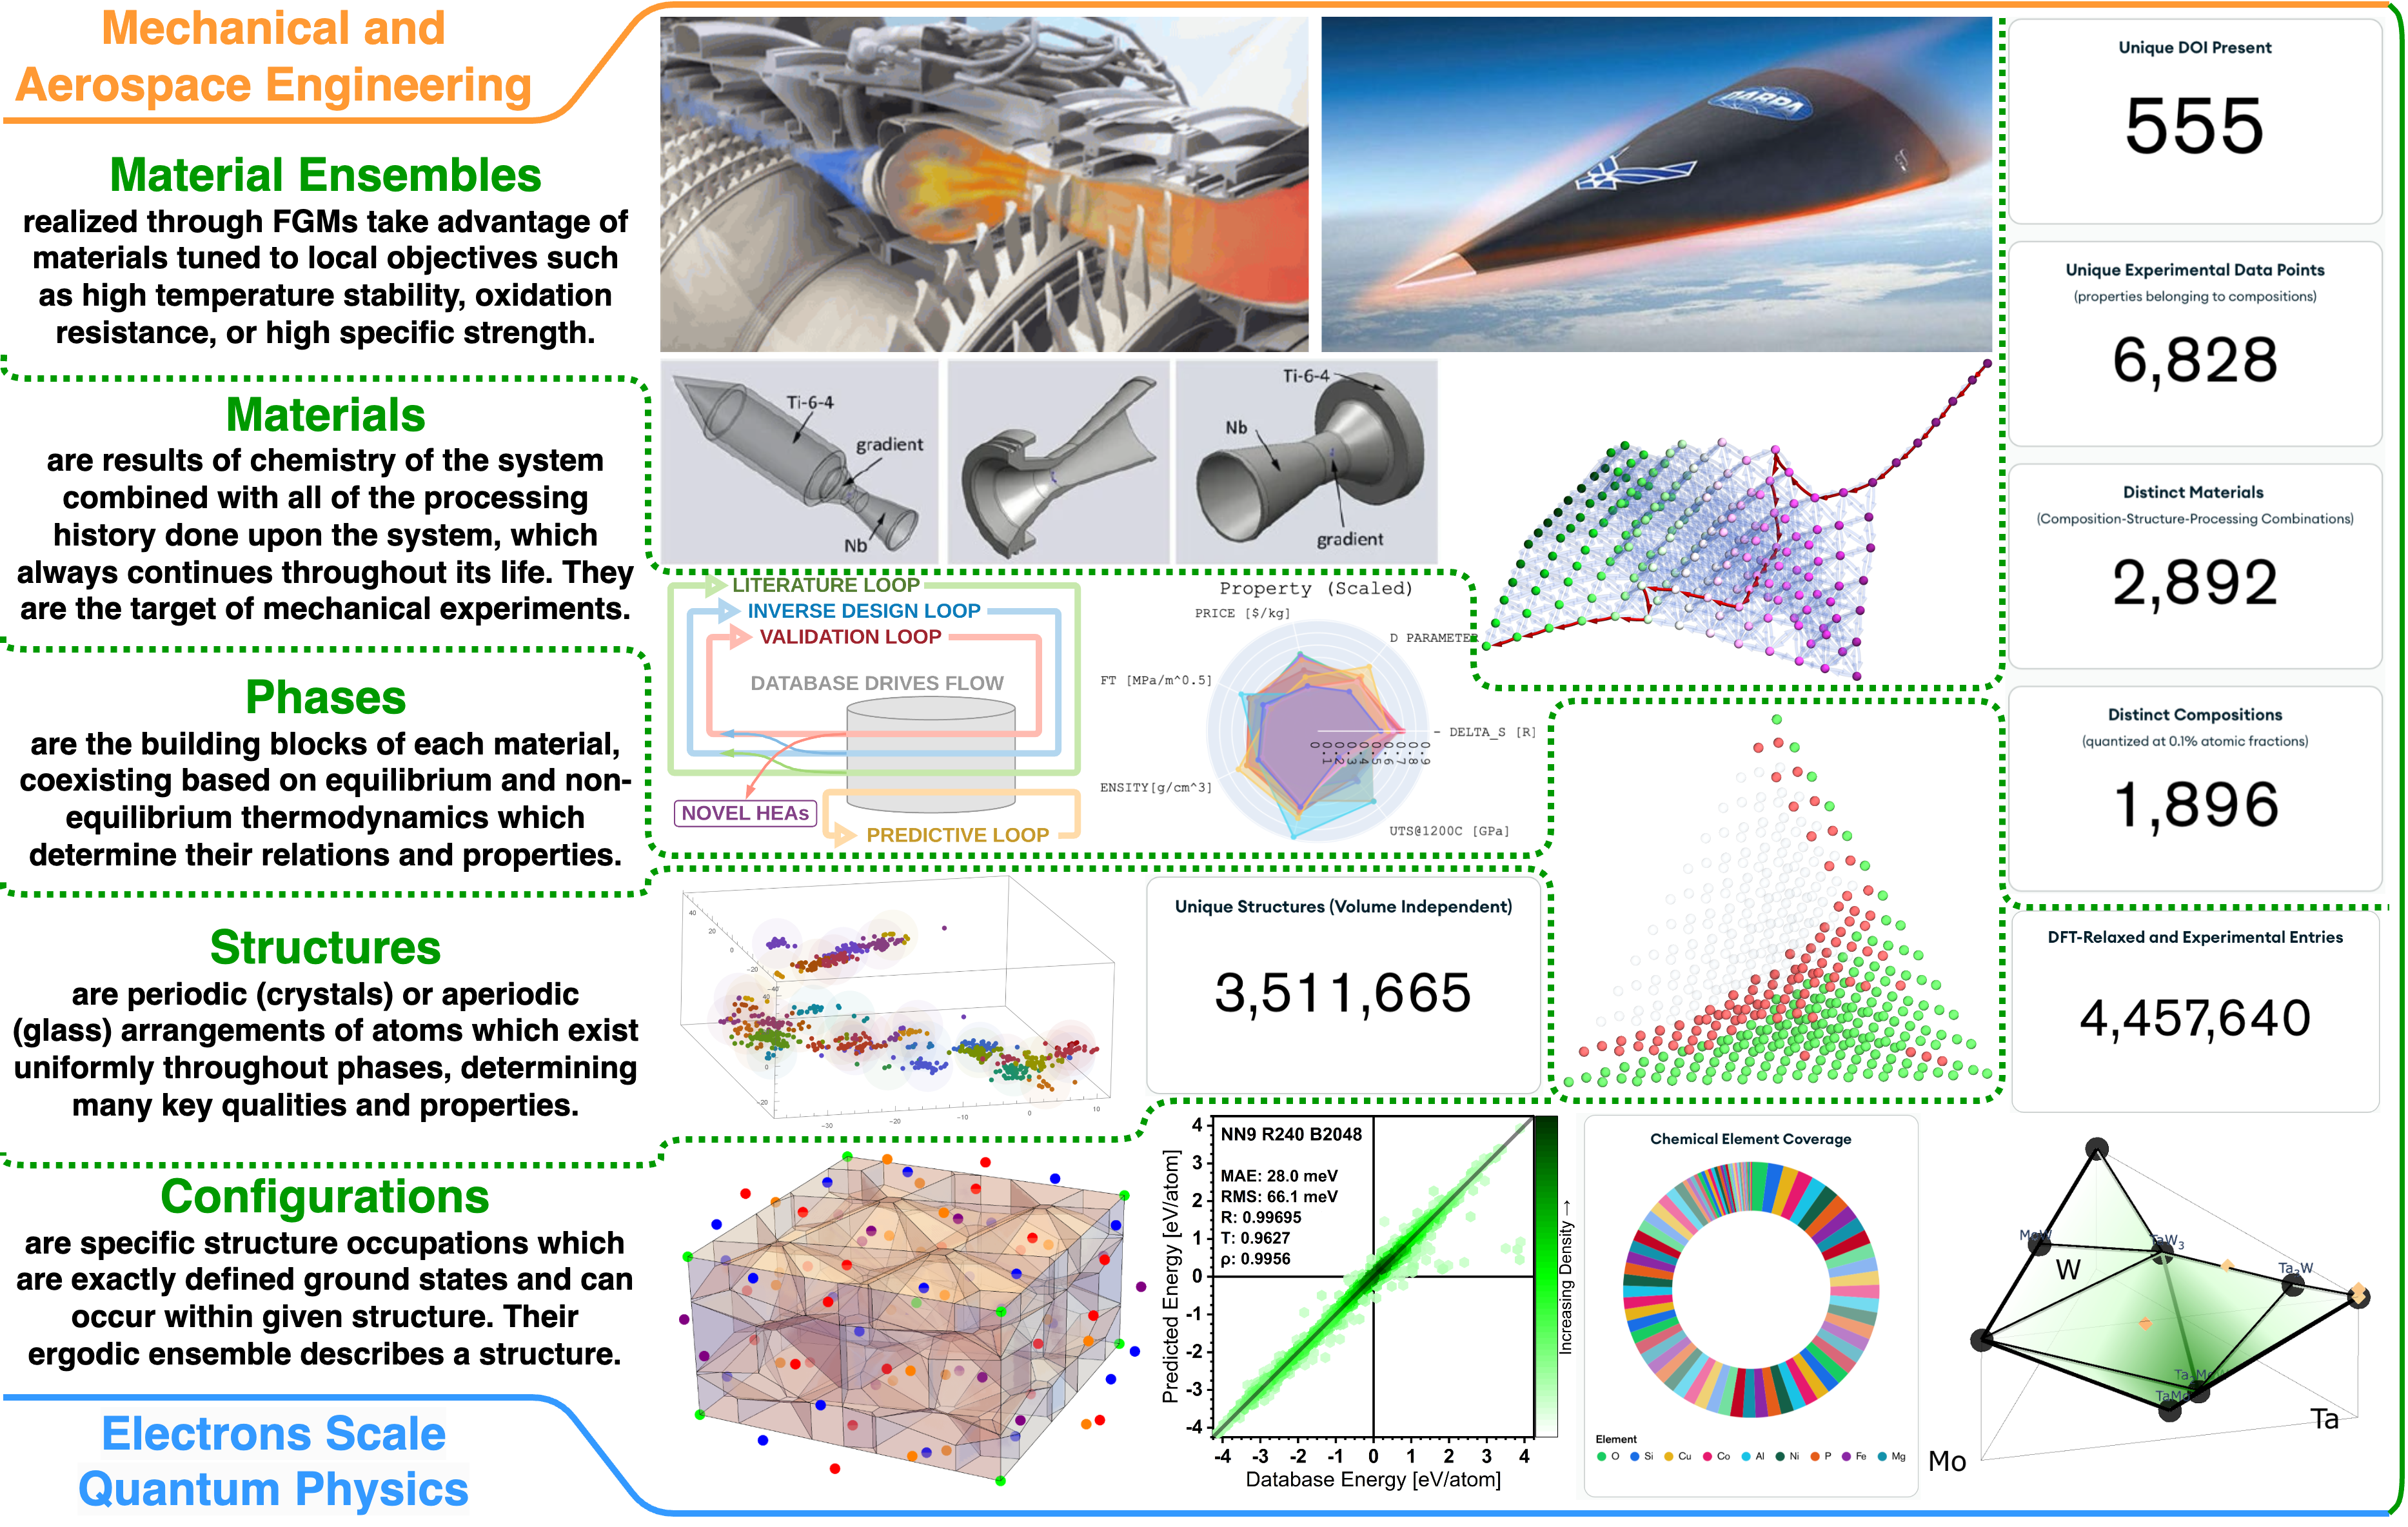
\includegraphics[width=0.95\textwidth]{intro/DissertationBigPicture.png}
    \caption{
    Intermediate material modeling scales bridging together quantum physics and aerospace engineering to enable high-technology solutions through excellence of underlying ensembles of materials. In this work, all of the scales are brought together to take advantage of data and knowledge from all relevant sources. Top render of hypersonic vehicle reproduced from DARPA under public domain and gray nozzle renders from \cite{Hofmann2014DevelopingManufacturing} under CC BY-NC-ND 4.0 License. Several images occur later in the manuscript in Figures \ref{pathplan:fig:lowgradientsquared}, \ref{ultera:fig:dashboard}, \ref{ultera:fig:dataloops}, \ref{inverse:fig:cgandemo}, \ref{infeasibilitygliding:fig:glide}, \ref{crystall:fig:ndbi2clusters}, \ref{pysipfenn:fig:ks2022}, \ref{sipfenn:fig:oqmdperformance}, and \ref{mpdd:fig:dataset}.
    }
    \label{intro:fig:bigpicture}
\end{figure}

Motivation 1:
Per DOE ARPA-E estimates, developing a standalone alloy which could continuously operate at $1300^oC$ has the potential to increase gas turbine efficiency up to 7\%, which will significantly reduce wasted energy and carbon emissions by saving up to 20 quads of energy in electricity generation and civilian aviation between now and 2050 \cite{ULTIMATEArpa-e.energy.gov}. Such efficiency increase could prevent release of approximately 1,000,000,000,000 kg of \ch{CO_2} from burning natural gas, or double that from coal.

Motivation 2:
Another extreme environment application is the class of hypersonic vehicles which travel faster than 5 times the speed of sound \emph{through Earth's atmosphere for extended periods of time}, thus, generating extreme sustained temperatures within structural components. This prompts the need for novel materials and engineering techniques, as evidenced by massive funding assigned to this research areas by United States military which increased its yearly budgets for hypersonic \emph{research} from \$3.8 billion in FY2022, to \$4.7 billion in FY2023, and to an undisclosed amount this year (FY2024) \cite{Sayler2024HypersonicCongress}.

\todo



\section{Flow of Material Discovery and This Work} \label{intro:sec:flow}

Throughout this work, all topics raised in Section \ref{intro:sec:bigpicture} will be discussed in a reversed order to progressively build from fundamentals to highly-specialized final applications, while retaining generality at every stage. This way, one will be able to build a holistic picture focused on how data flows within materials informatics research and converges together at consecutive length-scales to discover new materials in specific niches in a systematic, easy-to-automate approach, rather than build elaborate solutions that may \emph{happen} to work well but can also break the fundamentals - a common occurrence in our era of powerful computing and machine learning where tools \emph{always give an answer} but it may hold negative value.

As shown in Figure \ref{intro:fig:outline}, the first 4 chapters (colored blue) cover atomistic treatment of materials, discussing how data at this level is collected, featurized, managed and expanded. \texttt{SIPFENN} approach and the latest \texttt{pySIPFENN} featurization package are first developed. Then \texttt{MPDD} database with 4.5 million DFT-relaxed or experimentally observed entries is set up to serve as a highly efficient deployment vehicle. Lastly, \texttt{crystALL} approach automatically extends it into chemical areas of interest.

\begin{figure}[H]
    \centering
    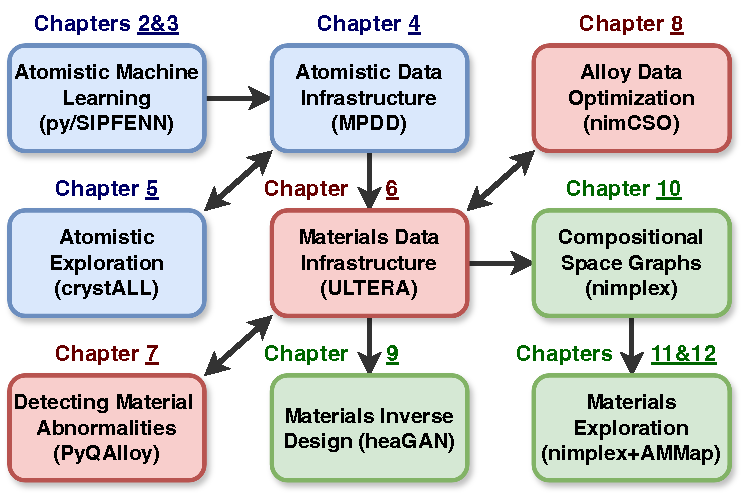
\includegraphics[width=0.7\textwidth]{intro/DissertationOutline.pdf}
    \caption{Schematic outline of this dissertation flowing through 3 overarching types of materials science research. It starts from atomistic treatment (blue) allowing modeling of physical materials (blue) and leading to design (green). For each category, three most significant advancements done in this work have been selected to showcase computational infrastructures and methods to extend our understanding or capabilities.}
    \label{intro:fig:outline}
\end{figure}

All of \texttt{MPDD} is then harvested to model materials at the physical scale by (1) serving as inputs to thermodynamic model generation using \texttt{pycalphad} \cite{Otis2017Pycalphad:Python} and \texttt{ESPEI} \cite{Bocklund2019ESPEICuMg} or training of \texttt{pySIPFENN} ML models generating needed data, and (2) informing experimental observations by, for instance, automatically compiling a set of carbides stable in an alloy system at 0K. At the same time, the largest experimental HEA data infrastructure, called \texttt{ULTERA}, is compiled joining together over 6,800 property datapoints manually extracted from 555 literature publications. 

The experimental database is curated through novel \texttt{PyQAlloy} package created to detect abnormalities and dramatically reduce fraction of erroneous data relative to other similar ones in the literature. Once curated, the \texttt{nimCSO} package can guide ML efforts in terms of which components of the data (chemical elements) should be considered when modeling to optimize trade-off between applicability and data density available to the models




\section{Executive Summary} \label{intro:sec:summary}

%%%%%%%%%%
First, Chapter \fullref{chap:sipfenn} introduces fundamental concepts critical to structure-informed modeling of atomic configurations from the perspective of machine learning (ML) modeling and presents design of such models employing artificial neural networks for the prediction of formation energies of atomic structures based on elemental and structural features of Voronoi-tessellated materials. It provide a concise overview of the connection between the machine learning and the true material-property relationship, how to improve the generalization accuracy by reducing overfitting, how new data can be incorporated into the model to tune it to a specific material system, and preliminary results on using models to preform local structure relaxations.

It results in three final models optimized for achieving (1) highest test accuracy on the Open Quantum Materials Database (OQMD), (2) high extrapolative performance in the discovery of new materials, and (3) high performance at a low computational cost. On a test set of 21,800 compounds randomly selected from OQMD, these models achieves a mean absolute error (MAE) of 28, 40, and 42 meV/atom, respectively. The first model represented the state-of-the-art performance on this problem when released in 2020 \cite{Krajewski2020SIPFENNModels} (see Table \ref{sipfenn:comparison-results}), the second model provides better predictions in a test case of interest not present in the OQMD, while the third one reduces the computational cost by a factor of 8 making it applicable to embedded and mobile applications. A transfer learning procedure was also demonstrated for the first time, showing dramatic improvements in extrapolation with just several datapoints (see Figure \ref{sipfenn:fig:transfersigmaVsDatapoints}).

The results were implemented into a new open-source tool called \texttt{SIPFENN} or \textit{Structure-Informed Prediction of Formation Energy using Neural Networks}, which not only improved the accuracy beyond existing models but also shipped in a ready-to-use form with pre-trained neural networks, which was first-of-a-kind at release, and a GUI interface allowing it be included in DFT calculations routines at nearly no cost.


%%%%%%%%
Next, Chapter \fullref{chap:pysipfenn} expands upon \texttt{SIPFENN} and implements a fully-featured machine learning focused analysis framework called \texttt{pySIPFENN} or \textit{python toolset for Structure-Informed Property and Feature Engineering with Neural Networks} to fuel needs of structure-informed materials informatics - a rapidly evolving discipline of materials science relying on the featurization of atomic structures or configurations to construct vector, voxel, graph, graphlet, and other representations useful for machine learning prediction of properties, fingerprinting, and generative design. This chapter discusses how current featurizers typically perform redundant calculations and how their efficiency could be improved by considering (1) fundamentals of crystallographic (orbits) equivalency to optimize ordered cases and (2) representation-dependent equivalency to optimize cases of dilute, doped, and defect structures with broken symmetry. It also discusses and contrasts ways of (3) approximating random solid solutions occupying arbitrary lattices under such representations.

Efficiency improvements discussed in this work were implemented within \texttt{pySIPFENN} and shown to increase performance from 2 to 10 times for typical inputs just based on fundamentals of materials science. Throughout this work, the authors explicitly discuss how these advances can be applied to different kinds of similar tools in the community.


%%%%%%%
Chapter \fullref{mpdd:sec:mpdd} shifts focus from developing new techniques for data analysis to building an innovative atomistic data infrastructure to fuel machine learning model training and deployment process. This effort builds from the idea that, fundamentally, each atomistic ML study comprises of three elements: a dataset or database of \emph{materials}, a \emph{descriptor} or set of features known for each material, and an ML algorithm trained to predict a \emph{property} or a set of them. These three are combined in two steps. First, the data representation is calculated using the descriptor. Then the model is iteratively evaluated on this representation or adjusted to improve it. Both processes are nearly instantaneous compared to ab-initio based methods; however, with extensive databases or materials modeled with large super-cells (e.g., glasses), compute times can grow into days or years for elaborate analysis tools deployed over many millions of datapoints. 

\texttt{MPDD} is a tool that can speed up the total process for the end-user by orders of magnitude through removal of the most time-intensive step, i.e., the descriptor calculation. To accomplish that, it moves from the traditional practice of sharing only the material-properties data to sharing the descriptors-properties data corresponding to the material as well, employing a high-performance NoSQL \texttt{MongoDB} database with highly engineered indexing system and fully salable compute node deployment model. The latter is used to progressively extend it based on guidance received from tools described in later chapters of this dissertation.

\texttt{MPDD} deployment model is not only much faster but also serves as a tool for an automated and robust embodiment of prior knowledge about materials in a graph-like fashion. Lastly, since the descriptors are often reused for related properties, our database provides a tremendous speed-up in the design space exploration.

Since 2023, a stable, well-implemented endpoint of the \texttt{OPTIMADE} API available at \href{https://optimade.mpdd.org}{https://optimade.mpdd.org} allows \texttt{MPDD} to be seamlessly integrated with other community databases and serve atomistic feature data associated with their entries for synergistic merger of experimental observations, ab initio calculations, and machine learning predictions.


%%%%%%%
Chapter \fullref{chap:crystall}, introduces a simple yet powerful approach to discovery of new atomic structures and identification of experimentally observed ones that evade identification, which was already demonstrated in certain important chemical systems. It implements in a concise computational tool which leverages millions of previously calculated structures from \texttt{MPDD} Database and other databases accessed through the \texttt{OPTIMADE} API to identify all atomic structures that can accommodate target stoichiometry (or uncertain chemical composition form experiments) and perform all permutations of substitutions to arrive at a list of tens of thousands of candidate structures. 

It analyzes candidates in the \texttt{KS2022} feature space, introduced in Chapter \ref{chap:pysipfenn} as part of \texttt{pySIPFENN}, to detect unique set of structures underlying different atomic configurations through different clustering techniques. Lastly, it selects a member from each cluster based on minimum formation energy to arrive at an ensemble of candidate configurations then passed to ab initio calculations or experiments for validation. 

Such ensemble approach is shown to provide critical advantages when contrasted with convex-hull-structure searching approach which recently dominated the community. It can also be used to expand unexplored regions of \texttt{MPDD} database, providing valuable deployment target for machine learning models.


%%%%%%%
Chapter \fullref{chap:ultera} crosses from the atomistic-level materials science into "real" materials physically created and measured experimentally, while still focusing on similar aspects of efficient modeling, data handing, and model deployment. It discusses the \texttt{ULTERA} Database, developed under the ARPA-E's ULTIMATE program and aimed at collecting literature data on high entropy alloys (HEAs).

\texttt{ULTERA} facilitates rapid discovery of new alloys using forward and inverse design, with the primary focus on creep behavior, yield stress, ductility, and hardness. Its advanced architecture, composed of many intermediate databases, pipelines, and analysis tools, is designed to automatically integrate starting literature data in real-time with methods such as experiments, generative modeling, predictive modeling, and validations. Thanks to such automation, the experimental team can operate on the best candidates available, while generation of new ones based on incoming experiments can be delegated to the cloud.

As of April 2024, ULTERA contains over 6,800 property-datapoints, corresponding to 2,900 unique HEAs, manually collected from 550 source literature publications. All data is available through a high-performance API, following FAIR principles.


%%%%%%%
Chapter \fullref{chap:pyqalloy} takes the \texttt{ULTERA} Database and dramatically increases its value to the machine learning applications by removing or fixing approximately 5\% of the errors present in it and other state-of-the-art HEA datasets, arriving at \emph{several times less erroneous data}.

In the past, these challenge was not as severe nor impactfull because the effort placed in the data analysis was much greater than data extraction; however, as our community moves towards this large-scale multi-source data collection, it increasingly starts to surface impacting ML efforts. While present in datasets on all alloy classes, this problem is particularly visible in high entropy alloys (HEAs) due to their novelty and complexity. A number of factors causes errors, including a lack of standardized notations and general parsing mistakes, such as typos, but most of them can be caught through detection of abnormalities in relation to the correct data and its patterns.

In this chapter, we present an open-source Python tool called \texttt{PyQAlloy} that can be run on alloy datasets to screen them for a variety of such abnormalities. It puts each data point in a variety of scopes ranging from individual datapoint analysis, through single-study meta-data, to the database as a whole.


%%%%%%%
Chapter \fullref{chap:nimcso} builds on top of \texttt{ULTERA} datasets curated by \texttt{PyQAlloy} and recognizes that selecting dimensions to model, or in this case, the selection of chemical elements to restrict the modeling effort, is a combinatorically hard problem for complex compositions existing in highly dimensional spaces due to the interdependency of components being present. Consequentially, optimizing the data availability and density for applications such as machine learning becomes a challenge.

A novel tool, called \texttt{nimCSO}, has been introduced and implmenets several methods for performing this task over even millions of datapoints and extreme dimensionalities encountered, for instance, in materials science of Compositionally Complex Materials (CCMs) which often span 20-45 chemical elements, 5-10 processing types, and several temperature regimes, for up to 60 total data dimensions.

It achieves the extreme performance by leveraging the metaprogramming ability of the Nim language to optimize itself at the compile time, both in terms of speed and memory handling, to the specific problem statement and dataset at hand based on a human-readable configuration file. As demonstrated in the chapter, it reaches the physical limits of the hardware (L1 cache latency) and can outperform an efficient native Python implementation over 400 times in terms of speed and 50 times in terms of memory usage (\emph{not} counting interpreter), while also outperforming NumPy implementation 35 and 17 times, respectively, when checking a candidate solution. It was designed to be both a user-ready tool and a scaffold for building even more elaborate methods in the future, including heuristics going beyond data availability. 


%%%%%%%
Chapter \fullref{chap:inversedesign} demonstrates how \texttt{ULTERA} dataset can be used to propose new alloys through inverse design. It leverages conditional Generative Adversarial Netowrks (cGAN) models to bias the predicted alloys in terms of (1) the property values by setting the conditioning and (2) the predicted compositions by recognizing \emph{concept vectors} in the latent space established at the training step. The former ability is implemented within a demonstrator Python package called \texttt{heaGAN} which can be used to design HEAs by setting design criteria. It also allows advanced users to re-train cGAN models based on their own data or a third-party property surrogate model.

%%%%%%%
Chapter \fullref{chap:nimplex} departs from both data and machine learning to focus on the mathematical abstractions of the alloy design problem. It begins by considering that many disciplines of science and engineering deal with problems related to compositions, ranging from chemical compositions in materials science to portfolio compositions in economics. They exist in non-Euclidean simplex spaces, causing many standard tools to be incorrect or inefficient, which is significant in combinatorically or structurally challenging spaces exemplified by Compositionally Complex Materials (CCMs) and Functionally Graded Materials (FGMs). In this chapter, we explore them conceptually in terms of problem spaces and quantitatively in terms of computational feasibility.

Several essential methods specific to the compositional (simplex) spaces are implemented, with most critical parts presented in chapter body as code listings, through a high-performance open-source library \texttt{nimplex}. Most significantly, we derive and implement an algorithm for constructing a novel n-dimensional simplex graph data structure, which contains all discretized compositions and all possible neighbor-to-neighbor transitions as pointer arrays. Critically, no distance or neighborhood calculations are performed, instead leveraging pure combinatorics and the ordering in procedurally generated simplex grids, keeping the algorithm $\mathcal{O}(N)$, so that graphs with billions of transitions take seconds to construct on a laptop. Furthermore, we demonstrate how such graph representations can be combined to express path-planning problem spaces and to incorporate prior knowledge while keeping the problem space homogeneous. This allows for efficient deployment of existing high-performance gradient descent, graph traversal search, and other path optimization algorithms.


%%%%%%%
Chapter \fullref{chap:infeasibilitygliding} leverages the novel graph-based representations of compositional spaces to dramatically improve our approach to screening and modifying compositionally complex alloys based on their structural constraint feasibility. It builds on the fact that the equilibrium existence of a particular phase in the phase-regions of chemical space (not necessarily corresponding to the present elements, as exploted in Chapter \ref{chap:nimplex}) is bound by a continuous surface of (generally) low curvature. Thus, performing the community-standard brute force screening type evaluation of all compositions will often calculate high numbers of points that cannot be reached.

Thus, \texttt{nimplex}-generated graphs are used to quickly re-implement the screening procedure into depth-first search traversals of the feasible regions that \emph{glide one the infeasibility boundaries}, reducing computation by half in semi-randomly picked "bad-case" which was known to produce relatively large feasible regions. In more elaborate screenings not taking advantage of prior knowledge, this improvement may very well reach between one and several orders of magnitude.


%%%%%%%
Lastly, Chapter \fullref{chap:pathplanning} takes additional advantage of the \texttt{nimplex}-generated graphs, which can be also extracted from feasible regions established in \ref{chap:infeasibilitygliding}, to deploy path planning algorithms and find sets of compositions that allow dissimilar alloys to be continuously combined in the least number of steps. Additional considerations are made in relation to an example property field of Root Mean Square Atomic Displacement (RMSAD) related to the yield stress in HEAs. In particular, its value, gradient, and magnitude of gradient are used to modify the graph weights encoding different design objectives, which are effortlessly solved with the same out-of-the box pathfinding approach.


%%%%%%%
Appendix \fullref{chap:supdiscussions} explores minor considerations tangential to the information flow or otherwise less critical, that may be of significant interest to some readers, while Appendix \fullref{chap:othersoft} discusses 8 pieces of software developed to during this work bur (1) were not directly used, (2) critical to discussion, or (3) were a contribution of a component to existing software.

Appendices \fullref{chap:nimplextutorial1} and \fullref{chap:nimplextutorial2} contain workshop material available under \texttt{nimplex} repository adapted to the formatting of this dissertation and go into details of both "Why?" and "How?" tools introduced between Chapters \ref{chap:nimplex} and \ref{chap:pathplanning} can be used by the end user. They can be run interactively with one-click cloud virtual environment by following current link at \href{https://nimplex.phaseslab.org}{nimplex.phaseslab.org} or by running them locally based on the supplementary materials.

Appendices \fullref{chap:pysipfenntutorial1} and \fullref{chap:pysipfenntutorial2} showcase how \texttt{pySIPFENN} integrates with other computational tools in the community and enables one to guide remote DFT calculations on a server cluster and adjust its models to a specific problem. Both were given by Adam Krajewski as guest lectures in the MatSE 580 course at Penn State in the Fall of 2023 and can be run interactively with one-click cloud virtual environment by following current link at \href{https://amkrajewski.github.io/MatSE580GuestLectures}{amkrajewski.github.io/MatSE580GuestLectures}, which also neatly presents the expected outcomes, or by running them locally based on the supplementary materials.

\printbibliography[heading=subbibintoc]


\chapter{Efficient Structure-Informed Featurization} \label{chap:pysipfenn}

Structure-informed materials informatics is a rapidly evolving discipline of materials science relying on the featurization of atomic structures or configurations to construct vector, voxel, graph, graphlet, and other representations useful for machine learning prediction of properties, fingerprinting, and generative design. This work discusses how current featurizers typically perform redundant calculations and how their efficiency could be improved by considering (1) fundamentals of crystallographic (orbits) equivalency to optimize ordered cases and (2) representation-dependent equivalency to optimize cases of dilute, doped, and defect structures with broken symmetry. It also discusses and contrasts ways of (3) approximating random solid solutions occupying arbitrary lattices under such representations.

Efficiency improvements discussed in this work were implemented within \texttt{pySIPFENN} or \textit{python toolset for Structure-Informed Property and Feature Engineering with Neural Networks} developed by authors since 2019 and shown to increase performance from 2 to 10 times for typical inputs. Throughout this work, the authors explicitly discuss how these advances can be applied to different kinds of similar tools in the community.

\section{Introduction} \label{pysipfenn:sec:Introduction}

\texttt{SIPFENN} or \textit{Structure-Informed Prediction of Formation Energy using Neural Networks} software, first introduced by the authors in 2020 \cite{Krajewski2022ExtensibleNetworks, Krajewski2020SIPFENNModels}, is one of several open-source tools available in the literature \cite{Ward2017, Jha2019IRNet, Chen2019GraphCrystals, Choudhary2021AtomisticPredictions, Deng2023CHGNetModelling, Davariashtiyani2023FormationRepresentation, Davariashtiyani2023FormationRepresentation, Schmidt2023Machine-Learning-AssistedMaterials} which train machine learning (ML) models on the data from large Density Functional Theory (DFT) based datasets like \texttt{OQMD} \cite{Saal2013MaterialsOQMD, Kirklin2015TheEnergies, Shen2022ReflectionsOQMD}, \texttt{AFLOW} \cite{Curtarolo2013AFLOW:Discovery, Toher2018TheDiscovery}, Materials Project \cite{Jain2013Commentary:Innovation}, NIST-\texttt{JARVIS}\cite{Choudhary2020TheDesign}, \texttt{Alexandria} \cite{Schmidt2022AFunctionals}, or \texttt{GNoME} \cite{Merchant2023ScalingDiscovery} to predict formation energies of arbitrary atomic structures, with accuracy high enough to act as a low-cost surrogate in the prediction of thermodynamic stability of ground and non-ground state configurations at 0K temperature. The low runtime cost allows such models to efficiently screen through millions of different atomic structures of interest on a personal machine in a reasonable time. 

In addition to high-accuracy neural network models trained on \texttt{OQMD} \cite{Saal2013MaterialsOQMD, Kirklin2015TheEnergies, Shen2022ReflectionsOQMD}, \texttt{SIPFENN} included a number of features not found in competing tools available at the time, such as the ability to quickly readjust models to a new chemical system based on just a few DFT data points through transfer learning and a selection of models optimized for different objectives like extrapolation to new materials instead of overfitting to high-data-density regions or low memory footprint \cite{Krajewski2022ExtensibleNetworks}.

\texttt{SIPFENN}'s usefulness has been demonstrated, for instance, in the cases where the structure of an experimentally observed compound could not be identified in industry-relevant Nd-Bi \cite{Im2022ThermodynamicModeling} and Al-Fe \cite{Shang2021FormingJoints} systems and had to be predicted. This was accomplished by (1) high-throughput generation of hundreds of thousands of possible candidates with the exact stoichiometry based on elemental substitutions into structures from both open DFT-based databases \cite{Saal2013MaterialsOQMD, Kirklin2015TheEnergies, Shen2022ReflectionsOQMD, Curtarolo2013AFLOW:Discovery, Toher2018TheDiscovery, Jain2013Commentary:Innovation, Choudhary2020TheDesign, Schmidt2022AFunctionals, Merchant2023ScalingDiscovery} and experimentally observed ones from Crystallography Open Database (COD) \cite{Grazulis2009CrystallographyStructures, Grazulis2012CrystallographyCollaboration, Grazulis2019CrystallographyPerspectives}, followed by (2) selection of thousands of low-energy candidates, (3) down-selection of tens of unique candidates based on clustering in the \texttt{SIPFENN}'s feature space, and (4) final validation with DFT and experiments. It has also been deployed in several thermodynamic modeling studies, e.g. of Nb-Ni system \cite{Sun2023ThermodynamicESPEI}, in conjunction with DFT and experimental data processed through \texttt{ESPEI} \cite{Bocklund2019ESPEICuMg} to automatically fit parameters of CALPHAD \cite{Olson2023GenomicDynamics} models deployed in \texttt{pycalphad} \cite{Otis2017Pycalphad:Python}.


\section{General Structure Featurization Improvements} \label{pysipfenn:sec:featurization}

\subsection{pySIPFENN Overview and Core Advantages} \label{pysipfenn:ssec:coreimprovements}

Being able to predict the thermodynamic stability of arbitrary atomic structures and their modifications is one of the most critical steps in establishing whether hypothetical candidates can be made in real life \cite{Zunger2019BewareMaterials}; however, it is certainly not the only task of interest to the community \cite{Jha2023MachineChallenges, Tao2021MachineDiscovery}. These diverse needs, combined with increasing interest in multi-property modeling, have shifted the focus of \texttt{SIPFENN} tool from model training \cite{Krajewski2022ExtensibleNetworks} toward the development of reliable, easy-to-use, and efficient general-purpose featurizers existing in a framework, which can be used by researchers and companies to quickly develop and deploy property-specific models, or use features directly in exploring similarity and trends in materials.

Thus, while the acronym has been retained, the name of the software has been changed to \textit{python toolset for Structure-Informed Property and Feature Engineering with Neural Networks} or \texttt{pySIPFENN}, and the software component has been carefully re-implemented in its entirety to make it as general as possible and enable the following core advantages:

\begin{enumerate}
    
    \item Reliable featurization, which can be immediately transferred to other tools thanks to standalone submodule implementations based only on two common libraries (\texttt{NumPy} \cite{Harris2020ArrayNumPy} and \texttt{pymatgen} \cite{Ong2013PythonAnalysis}). These include completely re-written \texttt{Ward2017} Java-based featurizer \cite{Ward2017} (see Section \ref{pysipfenn:ssec:Ward2017Translation}) and 3 new ones, described in Sections \ref{pysipfenn:sec:ordered}, \ref{pysipfenn:sec:dilute}, and \ref{pysipfenn:sec:randomsolutions}.

    \item Effortless plug-and-play deployment of neural network (and other) ML models (for any property) utilizing any of the defined feature vectors, enabled by the use of Open Neural Network Exchange (\texttt{ONNX}) open-source format \cite{Bai2019ONNX:Exchange} which can be exported from nearly every modern ML framework and is then loaded into \texttt{pySIPFENN}'s \texttt{PyTorch} backend \cite{Paszke2019PyTorch:Library} through \texttt{onnx2torch} \cite{Kalgin2021Onnx2torch:PyTorch}. Furthermore, implementing custom predictors, beyond those supported by \texttt{PyTorch}, is made easy by design.

    \item Dedicated \texttt{ModelExporters} submodule makes it easy to export trained models for publication or deployment on a different device while also enabling weight quantization and model graph optimizations to reduce memory requirements.

    \item The ability to acquire data and adjust or completely retrain model weights through automated \texttt{ModelAdjusters} submodule. Its applications include:
    \begin{enumerate}
        \item Fine-tuning models based on additional local data to facilitate transfer learning ML schemes of the domain adaptation kind \cite{Ben-David2010ADomains}, where a model can be adjusted to new chemistry and specific calculation settings, introduced by \texttt{SIPFENN} back in 2020 \cite{Krajewski2022ExtensibleNetworks}, which is also being adopted by other models like \texttt{ALIGNN} \cite{Gupta2024Structure-awareDatasets}. Such an approach can also be used iteratively in active learning schemes where new data is obtained and added.
        
        \item Tuning or retraining of the models based on other atomistic databases, or their subsets, accessed through \texttt{OPTIMADE} \cite{Andersen2021OPTIMADEData, Evans2024DevelopmentsExchange} to adjust the model to a different domain, which in the context of DFT datasets could mean adjusting the model to predict properties with DFT settings used by that database or focusing its attention to specific chemistry like, for instance, all compounds of Sn and all perovskites.
        
        \item Knowledge transfer learning \cite{Torrey2010HandbookLearning} to adjust models to entirely new, often less available properties while harvesting the existing pattern recognition.
    \end{enumerate}    
\end{enumerate}

The resulting \texttt{pySIPFENN} computational framework is composed of several components, as depicted in Figure \ref{pysipfenn:fig:pySIPFENNMainSchematic}, and is available through several means described in Section \ref{pysipfenn:sec:softwareavaialbility}, alongside high-quality documentation and examples.

\begin{figure}[h!]
    \centering
    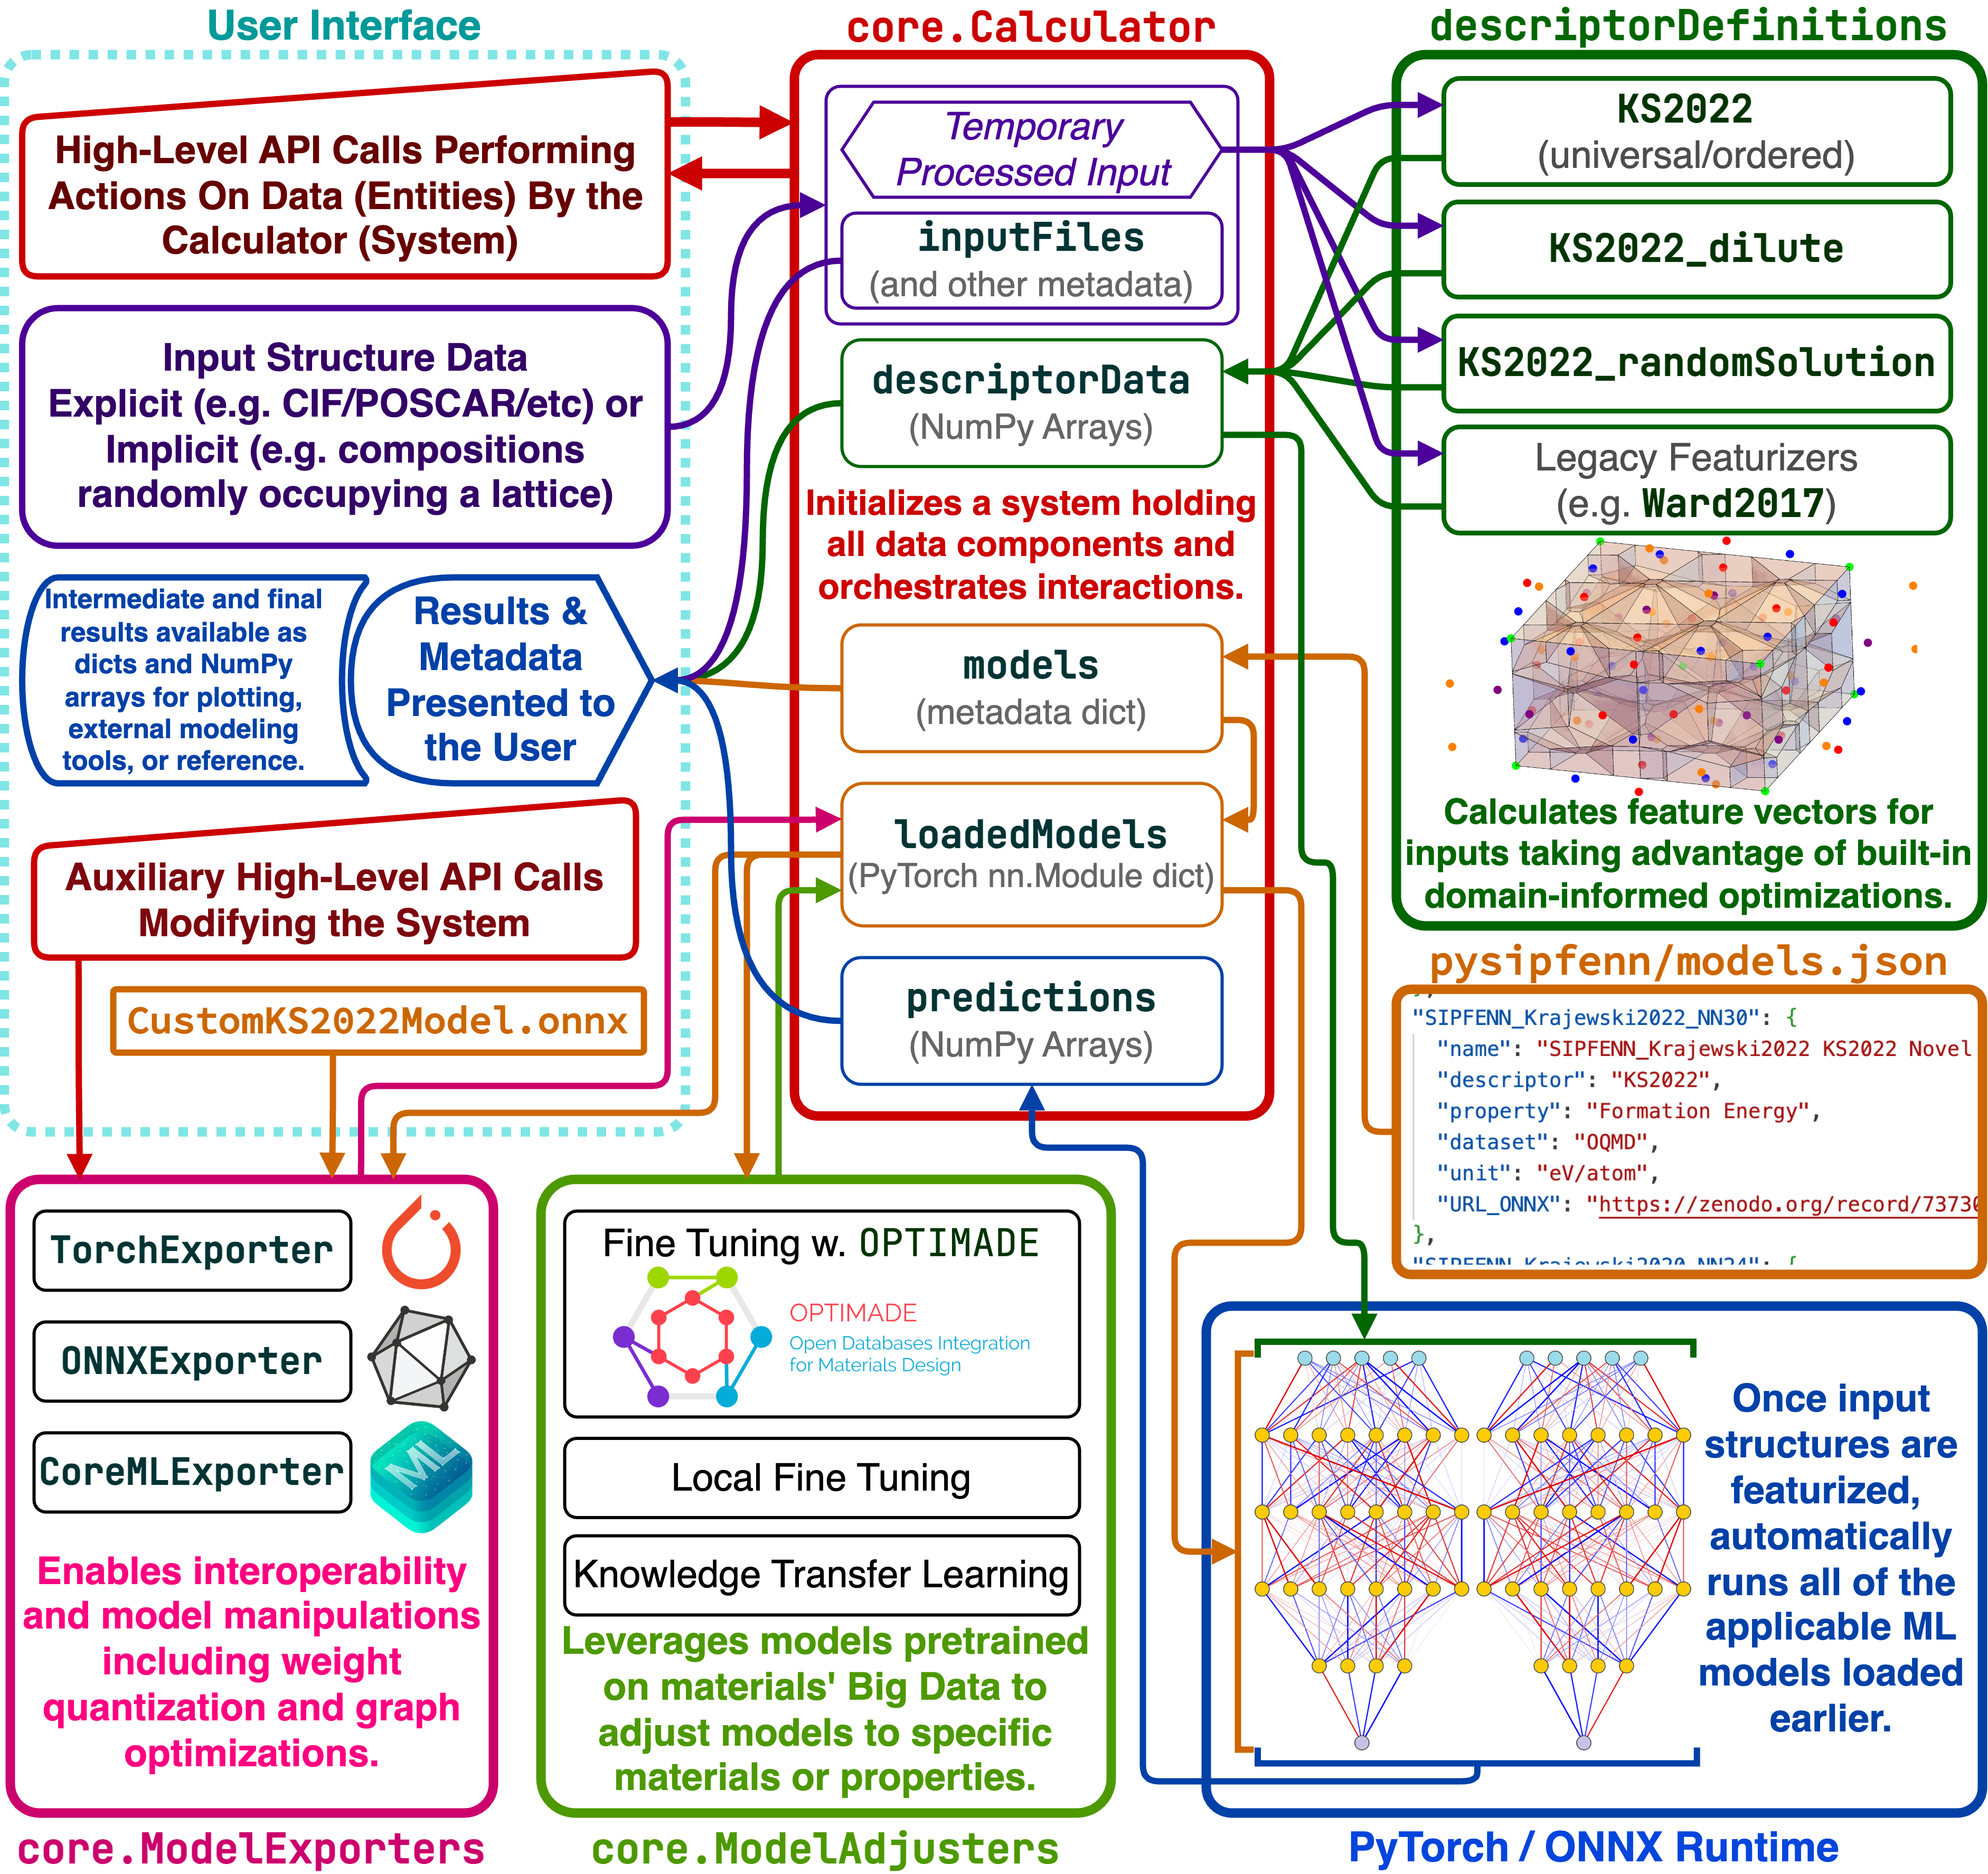
\includegraphics[width=0.85\textwidth]{pysipfenn/pySIPFENN_MainSchematic.png}
    \caption{Main schematic of \texttt{pySIPFENN} framework detailing the interplay of internal components described in Section \ref{pysipfenn:ssec:coreimprovements}. The user interface provides a high-level API to process structural data within \texttt{core.Calculator}, pass it to featurization submodules in \texttt{descriptorDefinitions} to obtain vector representation, then passed to models defined in \texttt{models.json} and (typically) run automatically through all available models. All internal data of \texttt{core.Calculator} is accessible directly, enabling rapid customization. An auxiliary high-level API enables advanced users to operate and retrain the models.}
    \label{pysipfenn:fig:pySIPFENNMainSchematic}
\end{figure}


\subsection{Ward2017 Reimplementation} \label{pysipfenn:ssec:Ward2017Translation}

In their 2017 work \citet{Ward2017} introduced a novel atomic structure featurization concept based on establishing and weighting neighbor interactions by faces from 3D Voronoi tesselation to describe local chemical environments (LCEs) of atomic sites and then performing statistics over them to obtain a global feature vector. The original \texttt{SIPFENN} models \cite{Krajewski2020SIPFENNModels} built on top of this while utilizing an improved, carefully designed deep neural network models to obtain up to 2.5 times lower prediction error on the same dataset \cite{Krajewski2022ExtensibleNetworks}. A detailed description of the descriptor can be found in Section 2.1 of \citet{Krajewski2022ExtensibleNetworks}. In general, the calculation of the \texttt{Ward2017} descriptor consists of three parts:

\begin{itemize}
    \item Calculation of attributes based upon global averages over the components of the structure.
    \item Calculation of attributes based upon local neighborhood averages for each site in the structure.
    \item Calculation of more complex attributes based upon averages over paths in the structure.
\end{itemize}

\citet{Ward2017} implemented the above calculations in Java, which was popular at the time; while most of the current machine-learning packages use almost exclusively Python (e.g., \texttt{scikit-learn} \cite{PedregosaFABIANPEDREGOSA2011Scikit-learn:Python} and \texttt{PyTorch} \cite{Paszke2019PyTorch:Library}), making it cumbersome to use Java. Even more critically, the original Java implementation was not computationally efficient (as explored in Sections \ref{pysipfenn:sec:ordered}, \ref{pysipfenn:sec:dilute}, and \ref{pysipfenn:sec:randomsolutions}), and enabling tools were not supported in Java.

In the present work, authors have reimplemented \citet{Ward2017} from scratch in Python as a standalone submodule for \texttt{pySIPFENN}, which calculates all 271 features within numerical precision, except for three performing a random walk on the structure, which is stochastic in nature and results in slightly different final values due to a different seed. The Voronoi tessellation has been implemented with \texttt{Voro++} \cite{Rycroft2007MultiscaleFlow, Rycroft2009Voro++:C++, Lu2023AnCells} and all numerical operations were written using \texttt{NumPy} \cite{Harris2020ArrayNumPy} arrays to greatly speed up the calculations and make the efficient utilization of different computing resources, such as GPUs, easy to implement.

\subsection{KS2022 Feature Optimization} \label{pysipfenn:ssec:ks2022features}

Typically, during feature engineering, researchers first attempt to collect all features expected to enable good inference and then remove some based on the interplay of several factors:
\begin{enumerate}
    \item \textbf{Low impact} on the performance, which increases the representation memory requirements and possibly increases the risk of overfitting to both systematic and random trends. 
    \label{pysipfenn:item:featureoptimize1}
    \item \textbf{High computational cost}, which limits the throughput of the method deployment.
    \label{pysipfenn:item:featureoptimize2}
    \item \textbf{Unphysical features or feature representations} which can improve model performance against well-behaving benchmarks covering a small subset of the problem domain but compromise model interpretability and extrapolation ability in unpredictable ways.
    \label{pysipfenn:item:featureoptimize3}
\end{enumerate}

The \texttt{KS2022} feature set, added in \texttt{pySIPFENN v0.10} in November 2022, is a significant modification of the \texttt{Ward2017} \cite{Ward2017}, which focuses on points \ref{pysipfenn:item:featureoptimize2} and \ref{pysipfenn:item:featureoptimize3} above, while enabling optimizations described in Sections \ref{pysipfenn:sec:ordered} through \ref{pysipfenn:sec:randomsolutions} and delegating the removal of low-impact features to modeling efforts and keeping featurization as problem-independent as possible.

First, all 11 features relying on representation of crystal symmetry space groups with space group number \texttt{float}s rather than classes (e.g. using one-hot vectors) have been removed due to the unphysical nature of such representation leading to, for instance, BCC ($229$) being much closer to FCC ($225$) than to just slightly uniaxially distorted BCC ($139$), which itself would be very close to trigonal structures. 

Next, featurization code has been thoroughly profiled in regard to time spent on the execution of feature-specific subroutines and analyzed in the context of feature importance identified in the past work \cite{Krajewski2022ExtensibleNetworks}. This led to the removal of the 1 \textit{CanFormIonic} feature, which relied on combinatorically expensive guessing of oxidation states, and 3 features based on Warren-Cowley (WC) parameters \cite{Cowley1950AnAlloys}, which were relatively very expensive without significantly contributing to the performance due to scarcity of disordered structures in most atomistic datasets. However, the authors intend to add them back in future problem-specific feature sets using a recently released high-performance library by \citet{Gehringer2023ModelsSimple}. 

Together, 15 features were removed, bringing the total number of the \texttt{KS2022} features to $256$ while disproportionately improving the featurization speed. For instance, in the case of featurization of 30 sites in a disordered (no symmetry) structure, \texttt{KS2022} is $2.3$ times faster than \texttt{Ward2017} ($430$ms vs $990$ms single-threaded on Apple M2 Max).

\section{Optimizations for Ordered Structures} \label{pysipfenn:sec:ordered}

Modeling of disordered materials is a critical area of research \cite{Zaki2023Glassomics:Intelligence}; however, the vast majority of atomistic ab initio datasets used for ML studies focuses on highly symmetric ordered structures because of their high availability and ability to model complex phenomena in a holistic fashion if local ergodicity can be established \cite{Liu2022TheoryTheorem, Liu2023ThermodynamicsPerspectives}. One evidence of the focus on such data is the fact that out of $4.4$ million atomic structures in \texttt{MPDD} \cite{Krajewski2021MPDD:Database}, which includes both DFT-based \cite{Saal2013MaterialsOQMD, Kirklin2015TheEnergies, Shen2022ReflectionsOQMD, Curtarolo2013AFLOW:Discovery, Toher2018TheDiscovery, Jain2013Commentary:Innovation, Choudhary2020TheDesign, Merchant2023ScalingDiscovery} and experimental \cite{Grazulis2009CrystallographyStructures, Grazulis2012CrystallographyCollaboration, Grazulis2019CrystallographyPerspectives} data, only $54$ thousand or $1.25\%$ lack any symmetry. It is also worth noting that this number used to be much lower before the recent publication of the \texttt{GNoME} dataset by Google DeepMind \cite{Merchant2023ScalingDiscovery}, which accounts for around $\frac{3}{4}$ of them. 

In the case of remaining $98.75\%$ structures, a 3-dimensional crystallographic spacegroup is defined for each of them along with corresponding \emph{Wyckoff positions} (designated by letters) which are populated with either zero (empty), one (when symmetry-fixed), or up to infinitely many (typically up to a few) atoms forming a set of symmetry-equivalent sites called \emph{crystallographic orbits} \cite{Muller2006RemarksPositions}. When these crystallographic orbits are collapsed into atoms occupying a unit cell, each is repeated 
based on the \emph{multiplicity} associated with the Wyckoff position it occupies, which can range from 1 up to 192 (e.g., position l in Fm-3m/225), with values 1, 2, 3, 4, 6, 8, 16, 24, 32, 48, and 96 being typical \cite{Mehl2016ThePrototypes} even in compositionally simple materials like one of the experimentally observed allotropes of pure silicon with atoms at the 8a, 32e, and 96g positions \cite{Gryko2000Low-densityGap}. For certain crystal lattice types, the multiplicity can be somewhat reduced by redefining their spatial periodicity with so-called \textit{primitive} unit cells, like in the case of the aforementioned Si allotrope, in which primitive unit cell has 4 times fewer (34) sites but still over 10 times more than the 3 unique crystallographic orbits.

This presents an immediate and previously untapped opportunity for multiplying the computational performance of most atomistic featurizers (e.g., \texttt{Matminer} \cite{Ward2018Matminer:Mining}) and ML models \cite{Ward2017, Chen2019GraphCrystals, Jha2019IRNet, Krajewski2022ExtensibleNetworks, Choudhary2021AtomisticPredictions, Deng2023CHGNetModelling, Davariashtiyani2023FormationRepresentation, Schmidt2023Machine-Learning-AssistedMaterials, Banik2024EvaluatingMaterials, Hu2021Atomtransmachine:Learning}, which nearly always process all atoms given in the input structure occasionally converting to primitive unit cell in certain routines (\texttt{CHGNet} \cite{Deng2023CHGNetModelling}), unless they operate on different occupancies of the same structure \cite{Crivello2022SupervisedExample}. This allows for a proportional decrease in both CPU/GPU time and memory footprint. The general-purpose \texttt{KS2022} in \texttt{pySIPFENN} uses high-performance symmetry analysis library \texttt{spglib} \cite{Togo2018Spglib:Search} to automatically take advantage of this whenever possible, as depicted in the schematic in Figure \ref{pysipfenn:fig:ks2022}. It shows an interesting example of a topologically close-packed $\sigma$ phase, which is critical to model in a wide range of metallic alloys \cite{Joubert2008CrystalPhase} but challenging in terms of combinatorics because of 5 unique sites that can be occupied by many elements \cite{Choi2019ADesign, Ostrowska2020ThermodynamicW} making it a very active area of ML modeling efforts \cite{Crivello2022SupervisedExample, Zha2024ApplyingEnergy} in the thermodynamics community.

\begin{figure}[h]
    \centering
    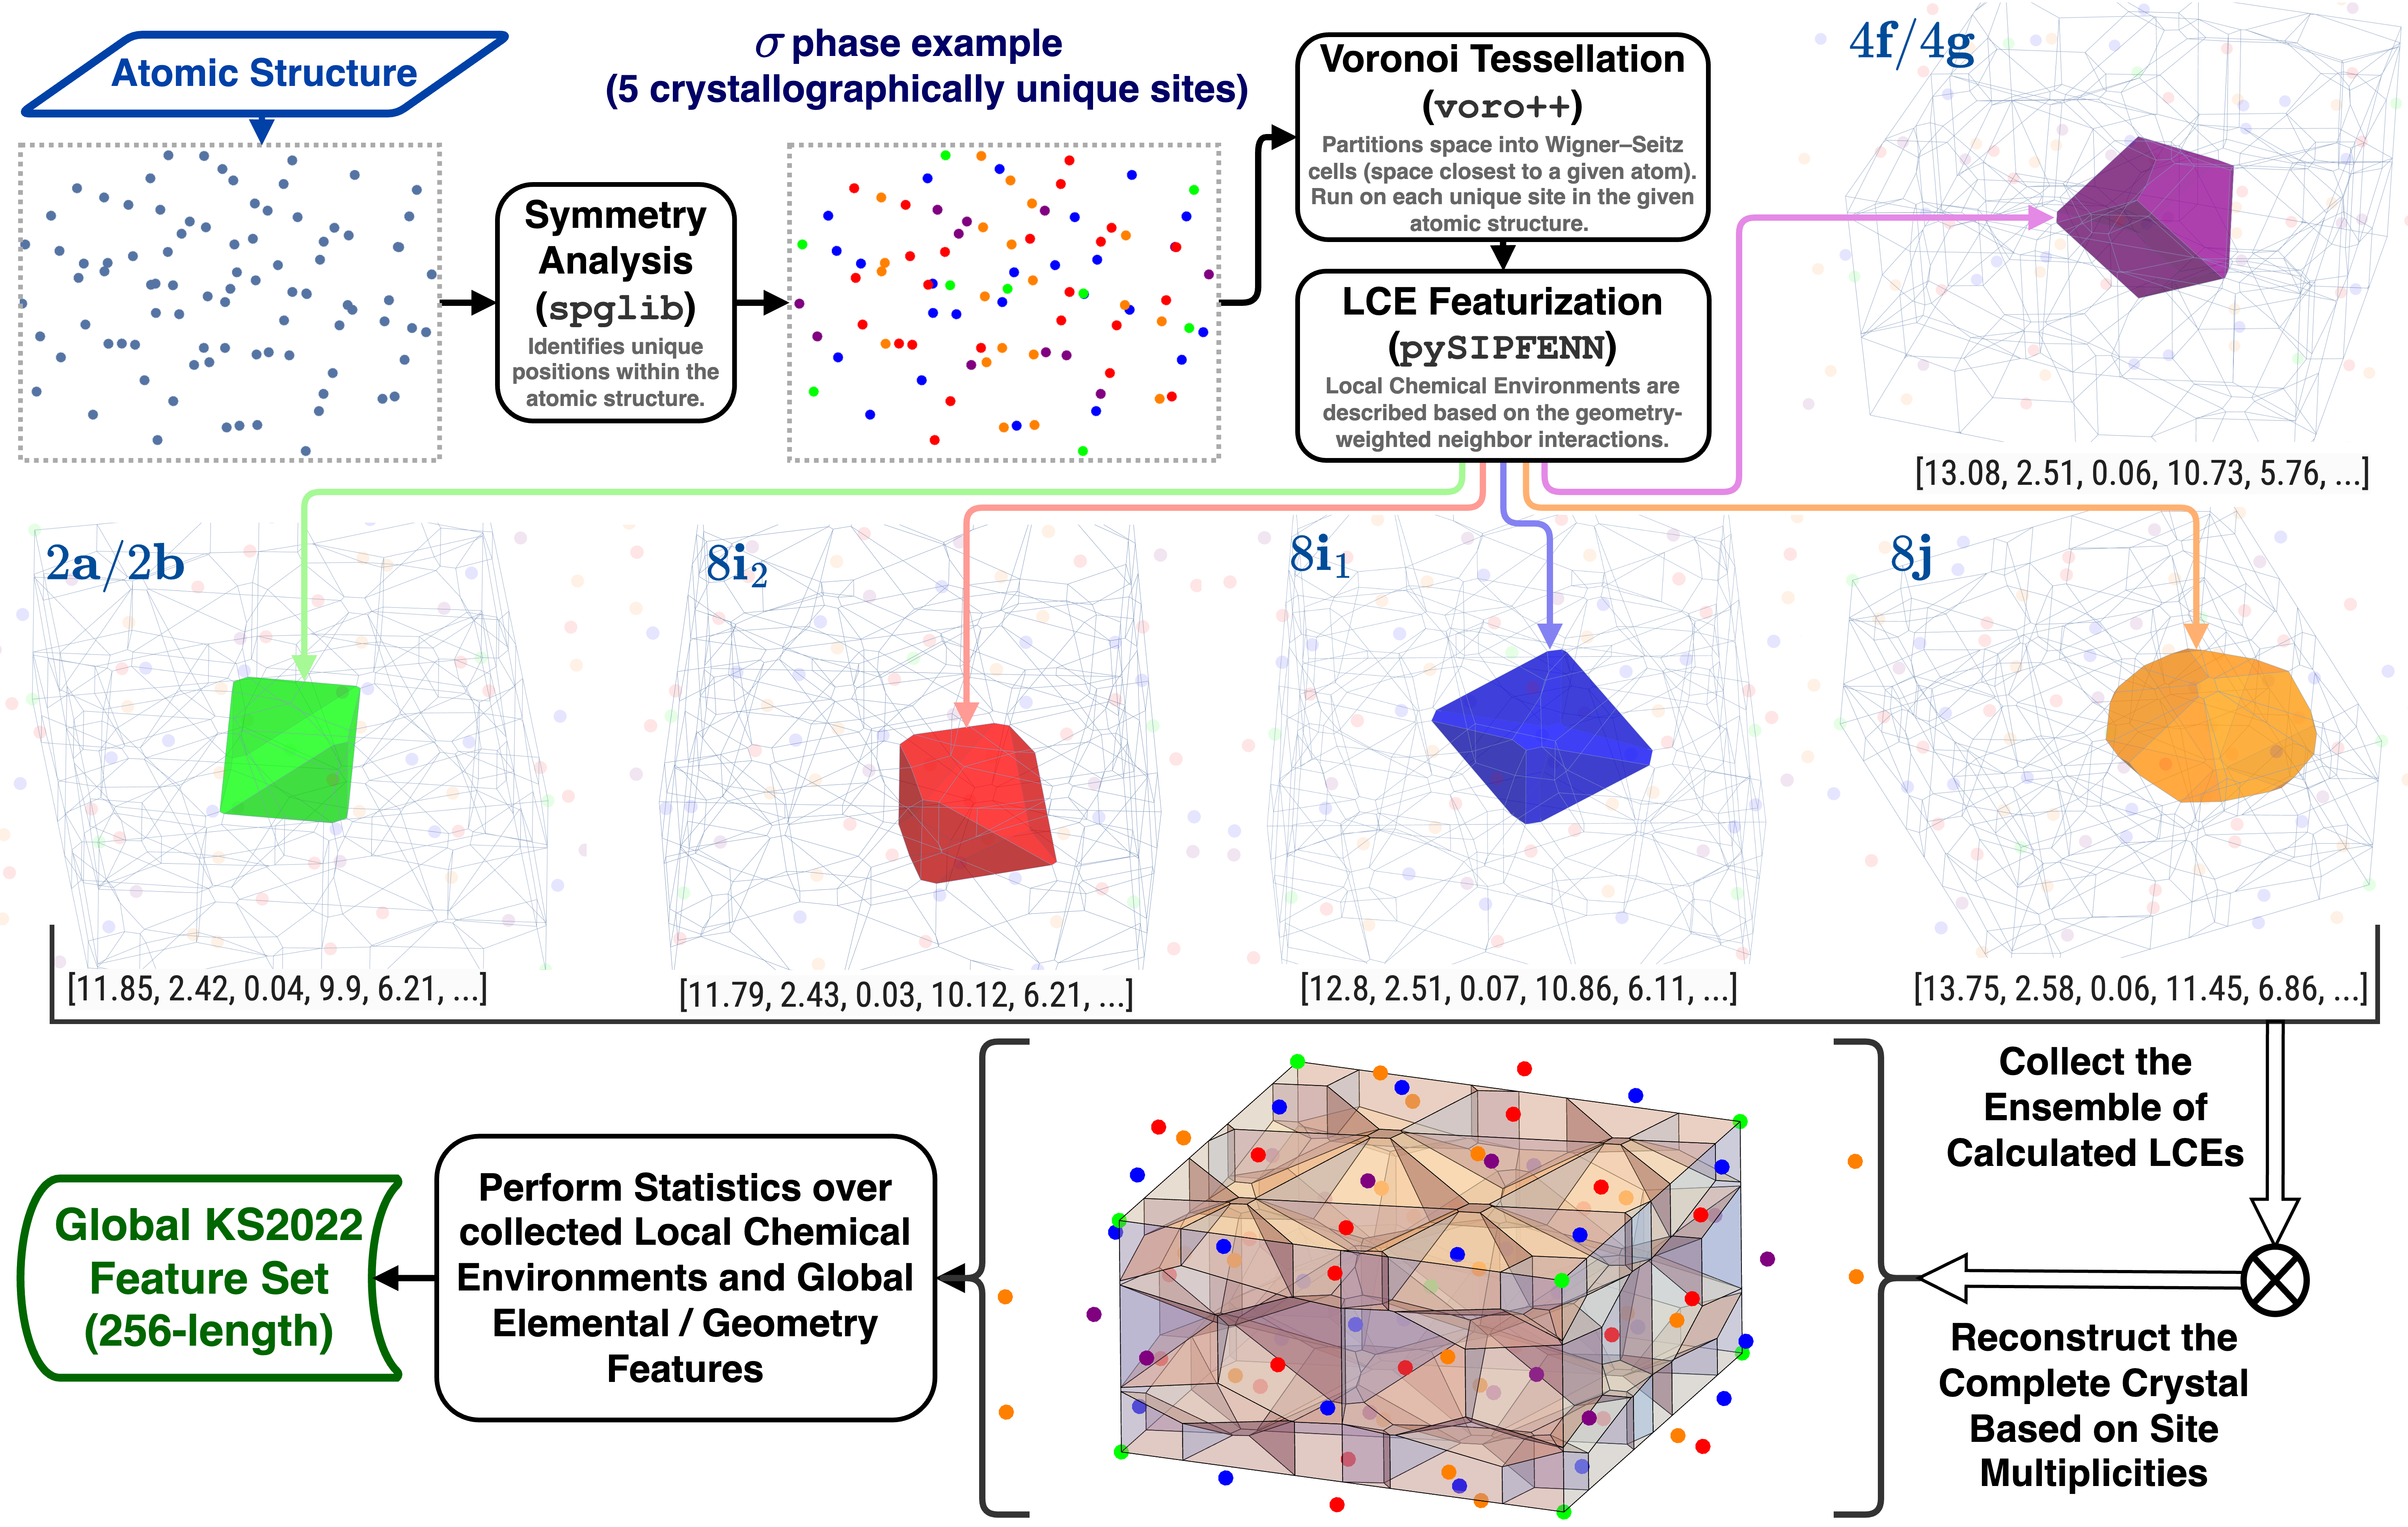
\includegraphics[width=0.98\textwidth]{pysipfenn/KS2022.png}
    \caption{
    Schematic of the general-purpose \texttt{KS2022} featurization routine with built-in optimization for ordered structures. First, the atomic structure (in \texttt{pymatgen Structure} object format \cite{Ong2013PythonAnalysis}) is loaded, and sites in it are annotated with their crystallographic orbits using \texttt{spglib} \cite{Togo2018Spglib:Search}. Then, one site is selected from each orbit to form a set of unique sites, for which Wigner-Seitz cells (depicted as colored polyhedra) are calculated with \texttt{Voro++} \cite{Rycroft2007MultiscaleFlow, Rycroft2009Voro++:C++, Lu2023AnCells} and featurized to get site-specific local chemical environment (LCE) descriptors. The complete site ensemble is then reconstructed based on multiplicities of Wyckoff positions corresponding to the sites. A non-trivial example of $\sigma$-phase with 30 atoms belonging to 5 crystallographic orbits with interesting Wigner-Seitz cells (relative to usually shown FCC/BCC ones \cite{Bohm1996VoronoiLattices}) has been depicted.
    }
    \label{pysipfenn:fig:ks2022}
\end{figure}

In the case of \texttt{KS2022} featurizer, running the same 30-atom test as in Section \ref{pysipfenn:ssec:ks2022features} but on $\sigma$ phase takes on average $84$ms or is 5.1 times faster thanks to processing 6 times less sites. Similar results should be (a) quickly achievable with any other featurizer processing individual sites, including most graph representations embedding local environments (e.g., \texttt{MEGNet} \cite{Chen2019GraphCrystals}) or deconstructing graphs into graphlets (e.g., \texttt{minervachem} molecule featurizer \cite{Tynes2024LinearCheminformatics}), and (b) possible with convolution-based models operating on graphs (e.g., \texttt{ALIGNN} \cite{Choudhary2021AtomisticPredictions}) or voxels \cite{Davariashtiyani2023FormationRepresentation} through custom adjustments to the specific convolution implementation. In the case of voxel representations and any other memory-intense ones, it may also be beneficial to utilize this approach to compress them when transferring between devices like CPU and GPU or across an HPC network.


\section{Optimizations for Dilute, Defect, and Doped Structures} \label{pysipfenn:sec:dilute}

The optimization strategy in Section \ref{pysipfenn:sec:ordered} ensures that only the sites that are \emph{guaranteed} to be \emph{crystallographically unique} are processed through featurization or graph convolution and is directly applicable to the vast majority of both data points and literature methods. However, in the case of methods relying on describing the immediate neighbors, whether through Wigner-Seitz cell (see Fig. \ref{pysipfenn:fig:ks2022}) or subgraph (see, e.g., \cite{Chen2019GraphCrystals}), one can achieve further efficiency improvements by considering which sites are \emph{guaranteed} to be \emph{unique under the representation}.

There are several classes of atomic structures where the distinction above makes a difference, but the room to improve is exceptionally high when one site in an otherwise highly symmetric structure is modified, leading to a structure that, depending on the context, will be typically called \emph{dilute} when discussing alloys \cite{Chong2021CorrelationAlloys}, \emph{doped} when discussing electronic materials \cite{Chen2022InteractionStudy}, or said to have \emph{defect} in a more general sense \cite{Castleton2009DensitySupercells}. Throughout \texttt{pySIPFENN}'s codebase and the rest of this work, the single term \emph{dilute} is used to refer to all of such structures due to authors' research focus on Ni-based superalloys at the time when optimizations below were made public in February 2023.

To visualize the concept, one can consider, for instance, a 3x3x3 body-centered cubic (BCC) conventional supercell (54 sites) and call it \textit{base structure}. If it only contains a single specie, then \texttt{KS2022} from Section \ref{pysipfenn:sec:ordered} will recognize that there is only one crystallographic orbit and only process that one. However, if a substitution is made at any of the 54 equivalent sites, the space group will change from Im-3m (229) to Pm-3m (221), with 8 crystallographic orbits on 7 Wyckoff positions; thus, the default \texttt{KS2022} featurizer will process 8 sites. 
At the same time, several of these crystallographic orbits will be differentiated \emph{only} by the orientation and distance to the dilute (substitution) site, which \emph{does} affect ab initio calculation results (e.g., vacancy formation energy vs supercell size \cite{Hargather2022ANi}), but is \emph{guaranteed} to \emph{have no effect on the model's representation} because of the exact same neighborhood configuration (including angles and bond lengths) if conditions given earlier are met. Thus, it only requires adjustments to the site multiplicities or convolution implementation (simplified through, e.g., a Markov chain). In the particular dilute-BCC example at hand, depicted in Figure \ref{pysipfenn:fig:KS2022dilute}, there are 4 such \emph{representation-unique} crystallographic orbits, i.e., 1 with the dilute atom, 2 neighboring the dilute atom sharing either large hexagonal (1st nearest neighbor shell) or small square face (2nd nearest neighbor shell), and 1 non affected by the dilute atom which is equivalent to the remaining 4 orbits; thus reducing number of sites that need to be considered by a factor of 2.

The \texttt{KS2022\_dilute} featurization routine, schematically depicted in Figure \ref{pysipfenn:fig:KS2022dilute}, conveniently automates the above process for both simple cases like aforementioned substitution in pure element and complex cases like introducing a dilute atom at the 2a/2b orbit in $\sigma$-phase (green cell in Fig. \ref{pysipfenn:fig:ks2022}), by performing independent identification of crystallographic orbits in the dilute structure and base structure, followed by identification of the dilute site and its configuration to establish orbit equivalency under \texttt{pySIPFENN}'s \texttt{KS2022} representation, to finally reconstruct complete site ensemble of the dilute structure.

\begin{figure}[h]
    \centering
    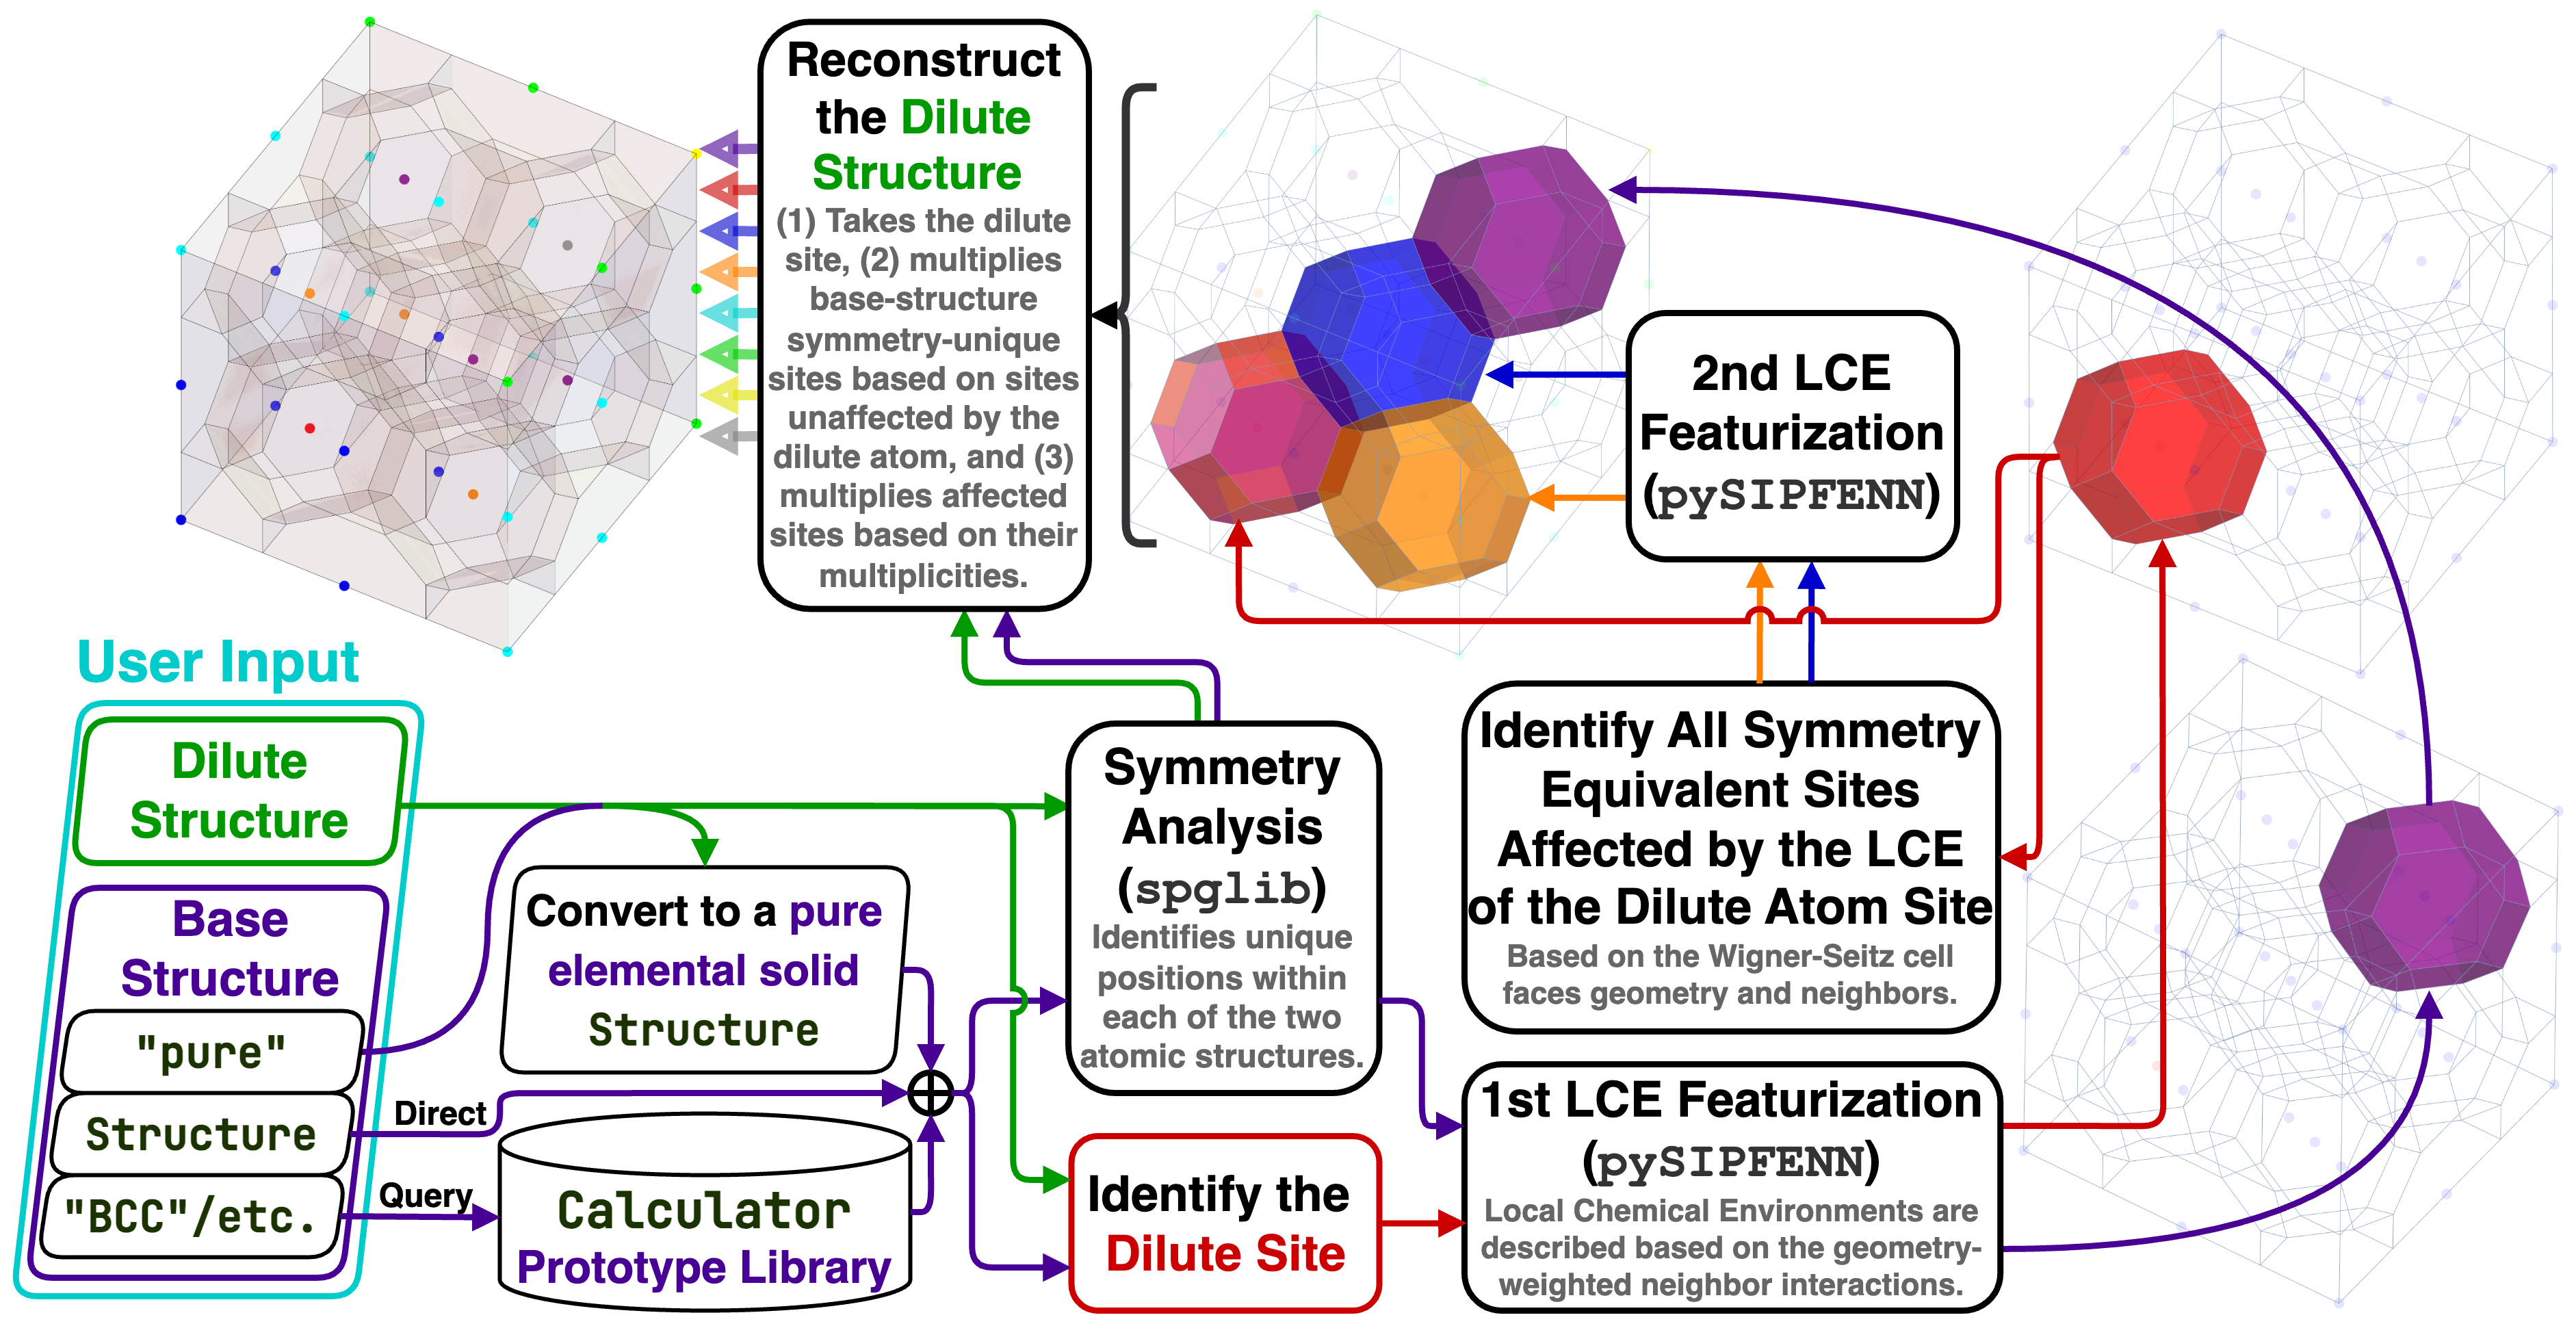
\includegraphics[width=0.85\textwidth]{pysipfenn/KS2022_dilute.png}
    \caption{Core schematic of the \texttt{KS2022\_dilute} featurizer. The dilute structure is compared to either the explicit or implicit base structure to identify the dilute site, which is then featurized alongside all crystallographically unique sites in the base structure. Information extracted from dilute structure featurization is then used to identify previously-equivalent sites affected by it, which go through the second round of featurization. Lastly, the complete ensemble is reconstructed, and \texttt{KS2022} are obtained. BCC supercell is used as an example.}
    \label{pysipfenn:fig:KS2022dilute}
\end{figure}

In the case of \texttt{KS2022\_dilute} implementation run on the dilute BCC supercell shown in Figure \ref{pysipfenn:fig:KS2022dilute}, the efficiency is improved nearly proportionally to the reduction in the number of considered sites, averaging $51$ms vs $98$ms \texttt{KS2022}, signifying 1.9 computational cost reduction relative to calculating all crystallographically unique sites. Or around 10-fold computational cost reduction relative to the standard \cite{Ward2017, Chen2019GraphCrystals, Jha2019IRNet, Krajewski2022ExtensibleNetworks, Choudhary2021AtomisticPredictions, Deng2023CHGNetModelling, Davariashtiyani2023FormationRepresentation, Schmidt2023Machine-Learning-AssistedMaterials} approach of processing all sites ($494$ms), while producing precisely the same results (within the numerical precision).


\section{Optimizations for Random Solid Solutions} \label{pysipfenn:sec:randomsolutions}

Sections \ref{pysipfenn:sec:ordered} and \ref{pysipfenn:sec:dilute} have demonstrated how recognition of symmetry in ordered structures can guarantee equivalency of sites and how understanding the character of featurization can further extend that notion of equivalency so that the ML representations of all sites can be obtained efficiently up to an order of magnitude faster. Random solid solutions are the conceptually opposite class of atomic structures, where the \emph{lack of} symmetry or site equivalency is \emph{guaranteed}, yet featurizing them requires one to solve the same problem of efficiently obtaining the ML representations of all sites present, which also happen to be infinite.

Typically, in the ab initio community, random solid solutions are represented using Special Quasirandom Structures (SQS) introduced in landmark 1990 work by \citet{Zunger1990SpecialStructures}, which are \emph{the} best structures to match neighborhood correlations in a purely random state given component ratios and number of atoms to use, hence the name \emph{special}. For many years, finding SQS structures required exponentially complex enumeration of all choices and was limited to simple cases until another critical work by \citet{VanDeWalle2013EfficientStructures}, which used simulated annealing Monte Carlo implemented through \texttt{ATAT} software to find these special cases much faster, exemplified through the relatively complex $\sigma$-phase and enabling the creation of SQS libraries used in thermodynamic modeling \cite{vandeWalle2017SoftwareData}.

However, the direct use of an SQS may not be the optimal choice for structure-informed random solid solution featurization due to several reasons. Firstly, as discussed by \citet{VanDeWalle2013EfficientStructures}, SQS can be expected to perform well on purely fundamental grounds for certain properties like total energy calculations, but one has to treat them with caution because different properties will depend differently on the correlation and selecting the SQS may be suboptimal. Building up on that, one could, for instance, imagine a property that depends strongly on the existence of low-frequency, high-correlation regions catalyzing a surface reaction or enabling nucleation of a dislocation. In terms of ML modeling, this notion is taken to the extreme with calculated features being both very diverse and numerous while being expected to be universal surrogates for such mechanistically complex properties.

Secondly, SQSs that can be generated in a reasonable time are limited in terms of the number of atoms considered, causing quantization of the composition. This is not an issue if a common grid of results is needed, e.g., to fit CALPHAD model parameters \cite{vandeWalle2017SoftwareData} or to train a single-purpose ML model \cite{Tandoc2023MiningAlloys}, but it becomes a critical issue if one needs to accept an arbitrary composition as the ML model and SQS would have to be obtained every time. This issue is further amplified by the rapidly growing field of compositionally complex materials (CCMs), which exist in vast many-component compositional spaces prohibiting SQS reuse even at coarse quantizations \cite{Krajewski2024Nimplex} while being a popular deployment target for both forward and inverse artificial intelligence methods \cite{Catal2023MachineProperties, Rao2022MachineDiscovery, Debnath2023ComparingAlloys} due to their inherent complexity.

Based on the above, it becomes clear that costly computing of an SQS structure would have to be done for every ML model, and it would not be consistent between chemistries and complexities. At the same time, the primary motivation for limiting the number of sites for ab initio calculations is gone since \texttt{KS2022} can featurize over 1,000 sites per second on a laptop (Apple M2 Max run in parallel). 

Thus, the objective of optimization is shifted towards consistency in convergence to feature vector values at infinity. To accomplish that, \texttt{pySIPFENN} goes back to random sampling but at a large scale and \emph{individually monitoring the convergence of every feature} during the expansion procedure, implemented through \texttt{KS2022\_randomSolutions} and depicted in Figure \ref{pysipfenn:fig:KS2022randomSolution}, to ensure individual convergence. 


\begin{figure}[h]
    \centering
    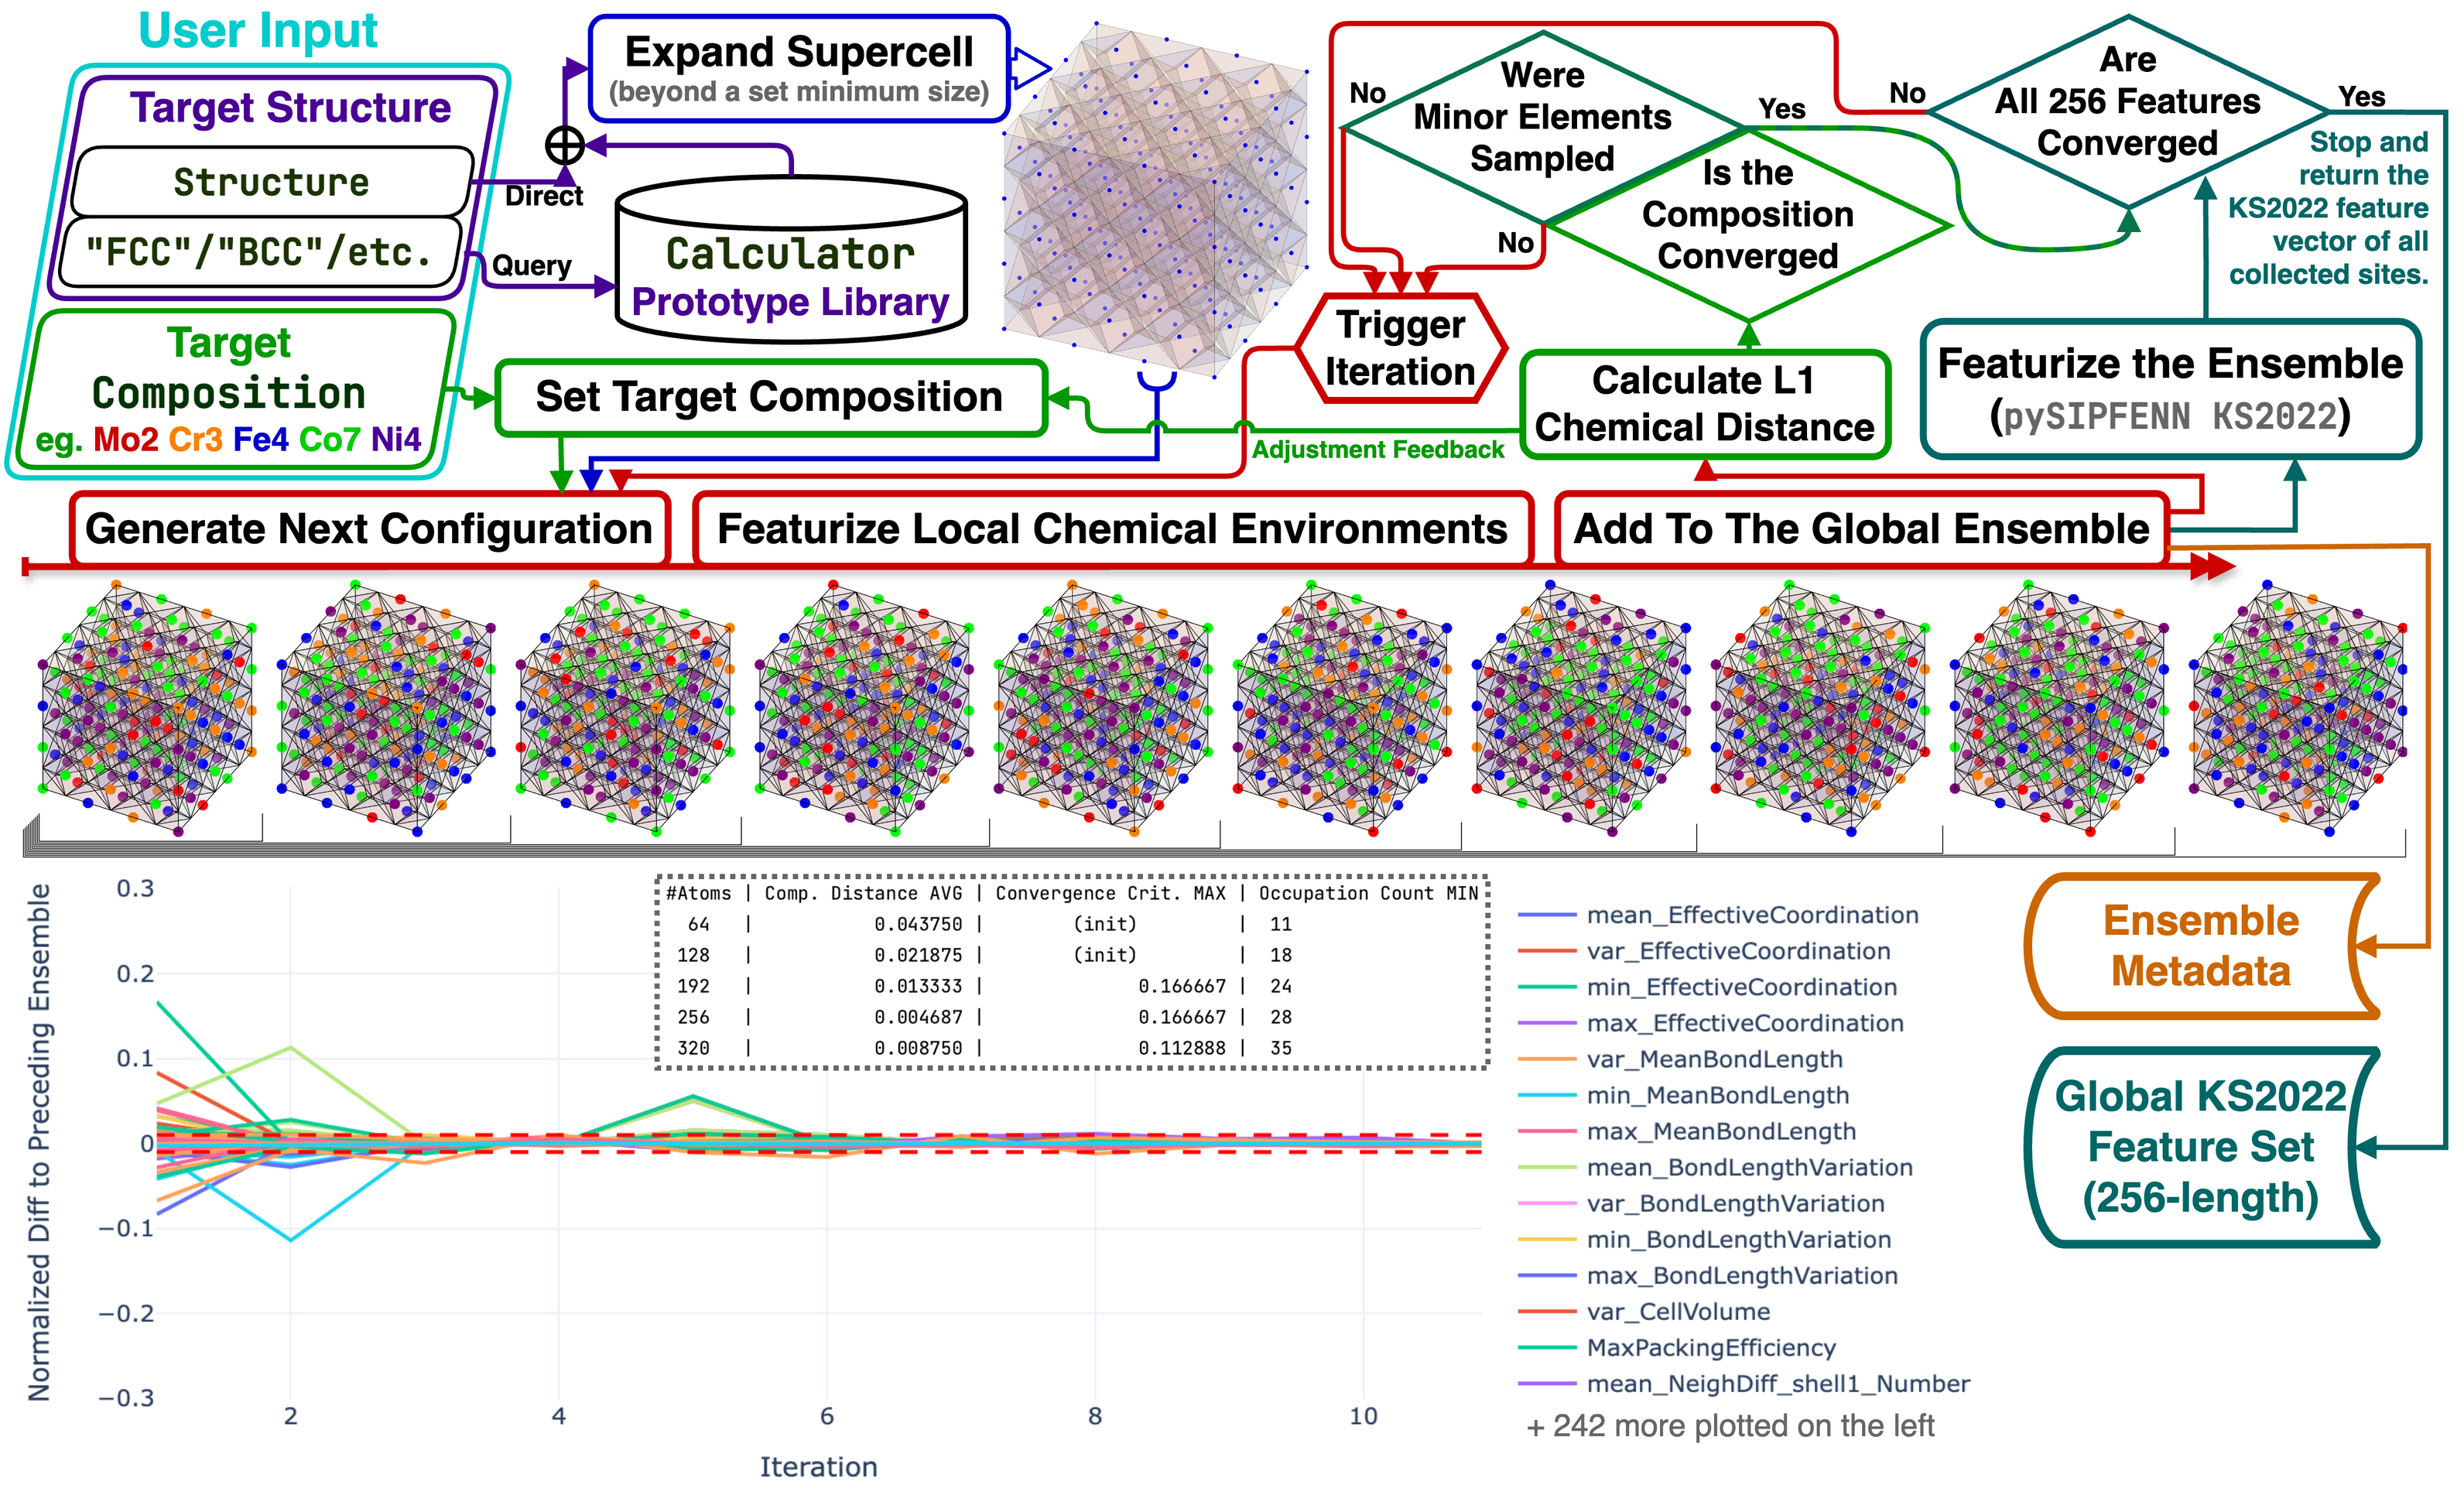
\includegraphics[width=0.95\textwidth]{pysipfenn/KS2022_randomSolution.png}
    \caption{
    Core schematic of the \texttt{KS2022\_randomSolutions} featurizer. The target structure given explicitly or implicitly is expanded to form a (lattice) (i.e. template) supercell. It is then iteratively populated with target composition (slightly adjusted each time) and divided into individual sites, which are featurized (like in \texttt{KS2022}) and added to the global ensemble. The process repeats until the composition is converged, all species have had a chance to occur, and \emph{every individual feature} has converged. Lastly, the global \texttt{KS2022} feature vector and metadata are returned. FCC supercell is used as an example.
    }
    \label{pysipfenn:fig:KS2022randomSolution}
\end{figure}

Such a representation-centered approach can also efficiently account for (1) the dissimilarity of any set of chemical elements and (2) the neighbor weight during featurization, where some may be much more important than others (see highly-anisotropic $\sigma$-phase Wigner-Seitz cells in Figure \ref{pysipfenn:fig:ks2022}). It is also flexible in accepting any target structure, even a distorted one, since no assumptions are made about the neighborhood geometry.

At the same time, it is important to note that such an approach is not a replacement for SQS in a general sense. It is, instead, a complementary method, as it does not result in a defined approximation of random structure but its representation for machine learning.

\section{Summary and Conclusions} \label{pysipfenn:sec:summaryconclusions}

\begin{itemize}
    \item \texttt{pySIPFENN} or \textit{python toolset for Structure-Informed Property and Feature Engineering with Neural Networks} is a free open-source software (FOSS) modular framework extending authors' past work \cite{Krajewski2022ExtensibleNetworks} described in Section \ref{pysipfenn:sec:Introduction} by including many key improvements in the structure-informed featurization, machine learning model deployment, different types of transfer learning (connected to OPTIMADE API \cite{Evans2024DevelopmentsExchange}), rewrite of key literature tools (e.g., \texttt{Ward2017} Java-based featurizer \cite{Ward2017}) into Python+\texttt{NumPy} \cite{Harris2020ArrayNumPy}, and optimizations of past feature set as described in Sections \ref{pysipfenn:ssec:coreimprovements}, \ref{pysipfenn:ssec:Ward2017Translation}, and \ref{pysipfenn:ssec:ks2022features}.
    
    \item \texttt{pySIPFENN} framework is uniquely built from tightly integrated yet highly independent modules to allow easy use of essential functions without limiting advanced researchers from taking specific components they need, like a specific featurizer, and simply copying it into their software, reducing dependencies to the minimum (including \texttt{pySIPFENN} itself).
    
    \item Section \ref{pysipfenn:sec:ordered} discusses how featurization of atomic structures (or configurations) to construct vector, voxel, graph, graphlet, and other representations is typically performed inefficiently because of redundant calculations and how their efficiency could be improved by considering fundamentals of crystallographic (orbits) equivalency to increase throughout of literature machine learning model, typically between 2 to 10 times. Critically, this optimization applies to $98.75\%$ of 4.4 million stored in \texttt{MPDD} \cite{Krajewski2021MPDD:Database}, which includes both DFT-based \cite{Saal2013MaterialsOQMD, Kirklin2015TheEnergies, Shen2022ReflectionsOQMD, Curtarolo2013AFLOW:Discovery, Toher2018TheDiscovery, Jain2013Commentary:Innovation, Choudhary2020TheDesign, Merchant2023ScalingDiscovery} and experimental \cite{Grazulis2009CrystallographyStructures, Grazulis2012CrystallographyCollaboration, Grazulis2019CrystallographyPerspectives} data, showing massive impact if deployed. \texttt{KS2022} featurizer implements these advances in \texttt{pySIPFENN} using \texttt{spglib} \cite{Togo2018Spglib:Search} and \texttt{Voro++} \cite{Rycroft2007MultiscaleFlow, Rycroft2009Voro++:C++, Lu2023AnCells}, while retaining ability to process arbitrary structures.
    
    
    \item Section \ref{pysipfenn:sec:dilute} explores how symmetry is broken in dilute, doped, and defect structures, to then discuss site equivalency under different representations and how this notion can be used to improve efficiency by skipping redundant calculations of sites which are not guaranteed to be equivalent based on crystallographic symmetry alone but need to be contrasted with defect-free representation. \texttt{KS2022\_dilute} featurizer implements these advances in \texttt{pySIPFENN}.

    \item Section \ref{pysipfenn:sec:randomsolutions} discusses featurization of perfectly random configuration of atoms occupying an arbitrary atomic structure and, for the first time, considers fundamental challenges with using SQS approach in the context of forward and inverse machine learning model deployment by extending past discussion on SQS limitations given by \citet{VanDeWalle2013EfficientStructures}, which do not typically appear in ab initio and thermodynamic studies. \texttt{KS2022\_randomSolutions} featurizer 
    has been developed to efficiently featurize solid solutions of any compositional complexity by expanding the local chemical environments (LCEs) ensemble until standardized convergence criteria are met.

    \item As described in Section \ref{pysipfenn:sec:softwareavaialbility}, software introduced in this work is continuously tested, well documented, regularly maintained, and 

    \item Throughout this work, the authors explicitly discuss how advances in featurization efficiency described in this work can be applied to different kinds of similar tools in the community, including those using voxel, graph, or graphlet representations.
    
\end{itemize}


\section{Software Availability and Accessibility} \label{pysipfenn:sec:softwareavaialbility}

\texttt{pySIPFENN} or \textit{python toolset for Structure-Informed Property and Feature Engineering with Neural Networks} is an easily extensible free, open-source software (FOSS) under \href{https://opensource.org/license/lgpl-3-0}{OSI-approved LGPL-3.0 license}, available as (1) source code hosted in a \texttt{GitHub} repository (\href{https://git.pysipfenn.org/}{git.pysipfenn.org}), (2) a python package through \href{https://pypi.org/project/pysipfenn/}{\texttt{PyPI} index}, and (3) a conda package hosted through \href{https://anaconda.org/conda-forge/pysipfenn}{\texttt{conda-forge} channel}.

It is very well-documented through (1) API reference, (2) detailed changelog, (3) install instructions, (4) tutorials and task-specific notes, and (5) FAQ, compiled for development (\href{https://pysipfenn.org/en/latest/}{pysipfenn.org/en/latest}), stable (\href{https://pysipfenn.org/en/stable/}{pysipfenn.org/en/stable}), and past (e.g., \href{https://pysipfenn.org/en/v0.12.0/}{pysipfenn.org/en/v0.12.0}) versions.

\texttt{pySIPFENN} has been built from the ground up to be a reliable user tool. It is automatically tested across a range of platforms (Linux / Windows / Mac (Intel) / Mac (M1)) and Python versions on every change, as well as on a weekly schedule.

It has been actively disseminated to its target audience through two large workshops organized with support from the Materials Genome Foundation (MGF / \href{https://materialsgenomefoundation.org}{materialsgenomefoundation.org}). The first one, covering \texttt{v0.10.3} and held online on March 2nd 2023, had over 300 users registered and over 100 following all exercises. It has been recorded and published on MGF's YouTube channel \cite{Krajewski20232023YouTube}. The second one, using \texttt{v0.12.1}, was held in-person on June 25th 2023 at the \href{https://calphad.org/calphad-2023}{CALPHAD 2023 conference} in Boston, as a part of Materials Genome Toolkit Workshops, covering its integration with \texttt{ESPEI} \cite{Bocklund2019ESPEICuMg} and \texttt{pycalphad} \cite{Otis2017Pycalphad:Python}. In November 2023, it was also employed in a pair of workshop-style graduate-level guest lectures introducing materials informatics (\href{https://amkrajewski.github.io/MatSE580GuestLectures/}{amkrajewski.github.io/MatSE580GuestLectures}), which can be used as an advanced tutorial.


\section*{Contributions}
\textbf{Adam M. Krajewski:} Conceptualization, Methodology, Software, Investigation, Writing - Original Draft, Validation, Visualization;
\textbf{Jonathan W. Siegel:} Software, Supervision, Writing - Review \& Editing;
\textbf{Zi-Kui Liu:} Funding acquisition, Supervision, Writing - Review \& Editing, Resources


\printbibliography[heading=subbibintoc]






\newpage
\chapter*{Vita}
\thispagestyle{empty}

Adam Krajewski was born in Europe, where he spent his childhood and received pre-college education at a public school nationally recognized for its university-level chemistry curriculum. He first came to the United States in 2013 and moved entirely in 2015, joining the Materials Science and Engineering Department at Case Western Reserve University. Within the first two months of enrollment, he began research in Prof. Welsch's group, and started to take graduate courses in his sophomore year. Around the same time, he joined Prof. Willard's group, progressively moving from experiments towards theory, modeling, and simulations. In late 2016, he enrolled in graduate courses in Artificial Intelligence and specialize in applying Machine Learning to his research problems in Materials Science. 

After earning his B.S.E. degree in 2019, he moved directly to pursue PhD at Penn State under world-renowned thermodynamics expert Prof. Zi-Kui Liu and had the pleasure of working on implementing a variety of computational techniques, including machine learning, while having the support of colleagues who are specialists in ab-initio modeling, thermodynamic calculations, and materials discovery. Since 2022, he also extensively collaborated with LLNL and have spent two summers on-site at the lab.

\end{document}
